\pdfminorversion=4 % necessary for EES
%% This template can be used to write a paper for
%% Computer Physics Communications using LaTeX.
%% For authors who want to write a computer program description,
%% an example Program Summary is included that only has to be
%% completed and which will give the correct layout in the
%% preprint and the journal.
%% The `elsarticle' style is used and more information on this style
%% can be found at 
%% http://www.elsevier.com/wps/find/authorsview.authors/elsarticle.
%%
%%
\documentclass[preprint,12pt]{elsarticle}

%%%%%%%%%%%%%%%%%%%%%%%%%%%%%%%%%%%%%%%%%%%%%%%%%%%%%%%%%%%%%%%%%%%%%
%% Place any additional packages needed here.  Only include packages
%% which are essential, to avoid problems later.
%%%%%%%%%%%%%%%%%%%%%%%%%%%%%%%%%%%%%%%%%%%%%%%%%%%%%%%%%%%%%%%%%%%%%

\usepackage[margin=1in]{geometry}

\usepackage[hyphens]{url}
%\usepackage{natbib}
\biboptions{sort&compress, square, comma}
\usepackage[breaklinks=true, linkcolor=blue, citecolor=blue, colorlinks=true]{hyperref}

\usepackage{graphicx}
\usepackage{caption}
\usepackage{subcaption}

\usepackage[version=3]{mhchem} % Formula subscripts using \ce{}, e.g., \ce{H2SO4}
\usepackage{bm}
\usepackage{latexsym, amsmath,amssymb}

\usepackage{mathtools}
% for larger sums
\usepackage{exscale, relsize}
\usepackage[retainorgcmds]{IEEEtrantools}

\usepackage{nicefrac}

\usepackage{booktabs,multicol}

% for math cancellation lines
\usepackage{cancel}
% to get nice text superscripts
\usepackage[super]{nth}

%better printing of numbers
\usepackage[T1]{fontenc}
\usepackage[english]{babel}
\usepackage{csquotes}
\usepackage{textcomp}

%my additions
%psuedo-code
\usepackage{algorithm}
\usepackage[noend]{algpseudocode}
%for sets
\usepackage{braket}
%abs and norm
\DeclarePairedDelimiter\abs{\lvert}{\rvert}%
\DeclarePairedDelimiter\norm{\lVert}{\rVert}% 
%set notation


%fix to dcases from here:http://tex.stackexchange.com/questions/252410/centering-in-dcases-environment/252414
\MHInternalSyntaxOn
\renewcommand{\dcases}
 {
  \MT_start_cases:nnnn
    {\quad}
    {$\m@th\displaystyle##$\hfil}
    {$\m@th\displaystyle##$\hfil}
    {\lbrace}
 }
\MHInternalSyntaxOff

% Swap the definition of \abs* and \norm*, so that \abs
% and \norm resizes the size of the brackets, and the 
% starred version does not.
\makeatletter
\let\oldabs\abs
\def\abs{\@ifstar{\oldabs}{\oldabs*}}
%
\let\oldnorm\norm
\def\norm{\@ifstar{\oldnorm}{\oldnorm*}}
\makeatother


\usepackage{siunitx}
\sisetup{group-separator={,},
     detect-all,
     binary-units,
     list-units = single,
     range-units = single,
     tophrase = --, 
     per-mode = symbol-or-fraction,
     separate-uncertainty = true,
     list-final-separator = {, and }
%    scientific-notation = fixed
}
\DeclareSIUnit\atm{atm}

\usepackage{fixltx2e}

\hyphenation{FORTRAN Fortran DRG-EP-SA DRG-ASA DRG-EP SEN-KIN CHEM-KIN}

% C++ macro
\def\CC{{C\nolinebreak[4]\hspace{-.05em}\raisebox{.4ex}{\footnotesize ++}}}
% derivative macros
\newcommand{ \ddt } [1] { \frac{ \partial #1 }{ \partial t } }
\newcommand{ \ddx } [1] { \frac{ \partial }{ \partial #1 } }
\newcommand{ \dydx } [2] { \frac{ \partial #1 }{ \partial #2 } }
\newcommand{ \ddydxx } [2] { \frac{ \partial^2 #1 }{ \partial #2^2 } }
\newcommand{\pluseq}{\mathrel{{+}{=}}}
\newcommand{\asteq}{\mathrel{{*}{=}}}

%to highlight text
%\usepackage{soul}
\usepackage[usenames, dvipsnames]{color}
%\newcommand{\hly}[1]{{\sethlcolor{yellow}\hl{#1}}}
%\newcommand{\hlb}[1]{{\sethlcolor{SkyBlue}\hl{#1}}}
%\newcommand{\hlg}[1]{{\sethlcolor{green}\hl{#1}}}

% Location for figures
\graphicspath{{./figures/}}

% Add [disable] option to quickly remove any
\usepackage[textsize=small,textwidth=2.5cm,disable]{todonotes}


% line numbers
%\usepackage{lineno}
%\newcommand*\patchAmsMathEnvironmentForLineno[1]{%
%  \expandafter\let\csname old#1\expandafter\endcsname\csname #1\endcsname
%  \expandafter\let\csname oldend#1\expandafter\endcsname\csname end#1\endcsname
%  \renewenvironment{#1}%
%     {\linenomath\csname old#1\endcsname}%
%     {\csname oldend#1\endcsname\endlinenomath}}% 
%\newcommand*\patchBothAmsMathEnvironmentsForLineno[1]{%
%  \patchAmsMathEnvironmentForLineno{#1}%
%  \patchAmsMathEnvironmentForLineno{#1*}}%
%\AtBeginDocument{%
%\patchBothAmsMathEnvironmentsForLineno{equation}%
%\patchBothAmsMathEnvironmentsForLineno{align}%
%\patchBothAmsMathEnvironmentsForLineno{flalign}%
%\patchBothAmsMathEnvironmentsForLineno{alignat}%
%\patchBothAmsMathEnvironmentsForLineno{gather}%
%\patchBothAmsMathEnvironmentsForLineno{multline}%

%}

%% This list environment is used for the references in the
%% Program Summary
%%
\newcounter{bla}
\newenvironment{refnummer}{%
\list{[\arabic{bla}]}%
{\usecounter{bla}%
 \setlength{\itemindent}{0pt}%
 \setlength{\topsep}{0pt}%
 \setlength{\itemsep}{0pt}%
 \setlength{\labelsep}{2pt}%
 \setlength{\listparindent}{0pt}%
 \settowidth{\labelwidth}{[9]}%
 \setlength{\leftmargin}{\labelwidth}%
 \addtolength{\leftmargin}{\labelsep}%
 \setlength{\rightmargin}{0pt}}}
 {\endlist}

\journal{Computer Physics Communications}

\begin{document}
\begin{frontmatter}

\title{\texttt{pyJac}: analytical Jacobian generator for chemical kinetics}

\author[osu]{Kyle~E.\ Niemeyer\corref{cor1}}
\ead{Kyle.Niemeyer@oregonstate.edu}

\author[uconn]{Nicholas~J.\ Curtis}
\author[uconn]{Chih-Jen Sung}

% addresses
\address[osu]{School of Mechanical, Industrial, and Manufacturing Engineering\\
  Oregon State University, Corvallis, OR 97331, USA}
\address[uconn]{Department of Mechanical Engineering\\
  University of Connecticut, Storrs, CT, 06269, USA}

\cortext[cor1]{Corresponding author}


%%%%%%%%%%%%%%%%%%%%%%%%%%%%%%%%%%%%%%%%%%%%%%%%%%%%%%%%%%%%%%%%%%%%%%
\begin{abstract}
% One or two sentence brief introduction to field
% Two or three sentences of detailed background
% One sentence clearly stating general problem
% One sentence summarizing main result ("here we show")
% Two or three sentences explaining what the main result reveals in direct comparison to what was thought to be the case previously, or how the main result adds to previous knowledge
% One or two sentences to put the results into a more general context
% Two or three sentences to provide a broader perspective
Accurate simulations of combustion phenomena require the use of detailed chemical kinetics in order to capture limit phenomena such as ignition and extinction as well as predict pollutant formation.
However, the chemical kinetic models for hydrocarbon fuels of practical interest exhibit both mathematical stiffness in the governing differential equations and large numbers of species and reactions, particularly for larger molecules.
In order to integrate the stiff equations governing chemical kinetics, generally reactive-flow simulations rely on implicit algorithms that require frequent Jacobian matrix evaluations; in addition, various computational combustion diagnostics methods require accurate Jacobian matrices.
Typically, finite differences numerically approximate these, but for larger chemical kinetic models this poses significant computational demands since the number of chemical source term evaluations scales with the square of species count.
Furthermore, existing analytical Jacobian tools do not optimize evaluations or support emerging SIMD processors such as GPUs.
Here we introduce \texttt{pyJac}, a Python-based open-source program that generates analytical Jacobian matrices for use in chemical kinetics modeling and analysis.
In addition to producing the necessary customized source code for evaluating reaction rates (including all modern reaction rate formulations), the chemical source terms, and the Jacobian matrix, \texttt{pyJac} uses an optimized evaluation order to minimize computational and memory operations.
First, we establish the correctness of the Jacobian matrices for kinetic models of hydrogen, methane, and ethylene oxidation (number of species ranging \SIrange{13}{111}) by showing agreement within \SI{1}{\percent} of high-order finite difference approximations.
We then demonstrate the performance, via matrix evaluation timing comparisons, achievable on CPUs and GPUs using \texttt{pyJac}.
% by optimizing the order of matrix element calculations.
%Finally, we explore the sparsity and characteristics of Jacobian matrices for these chemical kinetic models.
The Jacobian matrix generator we describe here will be useful for reducing the cost of integrating chemical source terms with implicit algorithms in particular and algorithms that require an accurate Jacobian matrix in general.
Furthermore, the open-source release of the program and Python-based implementation will enable wide adoption.
\end{abstract}

\begin{keyword}
Chemical kinetics \sep Jacobian \sep SIMD \sep GPU
\end{keyword}

\end{frontmatter}

%\linenumbers
%\renewcommand\linenumberfont{\normalfont\tiny}



%%%%%%%%%%%%%%%%%%%%%%%%%%%%%%%%%%%%%%%%%%%%%%%%%%%%%%%%%%%%%%%%%%%%%%
% Computer program descriptions should contain the following
% PROGRAM SUMMARY.

{\bf PROGRAM SUMMARY}
  %Delete as appropriate.

\begin{small}
\noindent
{\em Manuscript Title:} \texttt{pyJac}: analytical Jacobian generator for chemical kinetics \\
{\em Authors:} Kyle E.\ Niemeyer, Nicholas J.\ Curtis, Chih-Jen Sung \\
{\em Program Title:} pyJac                                    \\
{\em Journal Reference:}                                      \\
  %Leave blank, supplied by Elsevier.
{\em Catalogue identifier:}                                   \\
  %Leave blank, supplied by Elsevier.
{\em Licensing provisions:}                                   \\
  %enter "none" if CPC non-profit use license is sufficient.
{\em Programming language:} Python                            \\
{\em Computer:} Any                                              \\
  %Computer(s) for which program has been designed.
{\em Operating system:} Any (Linux, OS X, Windows)            \\
  %Operating system(s) for which program has been designed.
{\em RAM:} bytes                                              \\
  %RAM in bytes required to execute program with typical data.
%{\em Number of processors used:}                              \\
%  %If more than one processor.
%{\em Supplementary material:}                                 \\
%  % Fill in if necessary, otherwise leave out.
{\em Keywords:} Chemical kinetics, Jacobian  \\
  % Please give some freely chosen keywords that we can use in a
  % cumulative keyword index.
{\em Classification:} 16.12, 4.3                                \\
  %Classify using CPC Program Library Subject Index, see (
  % http://cpc.cs.qub.ac.uk/subjectIndex/SUBJECT_index.html)
  %e.g. 4.4 Feynman diagrams, 5 Computer Algebra.
{\em External routines/libraries:}                            \\
  % Fill in if necessary, otherwise leave out.
%{\em Subprograms used:}                                       \\
%  %Fill in if necessary, otherwise leave out.
{\em Nature of problem:}\\
  %Describe the nature of the problem here.
   \\
{\em Solution method:}\\
  %Describe the method solution here.
   \\
%{\em Restrictions:}\\
%  %Describe any restrictions on the complexity of the problem here.
%   \\
%{\em Unusual features:}\\
%  %Describe any unusual features of the program/problem here.
%   \\
{\em Additional comments:}\\
  %Provide any additional comments here.
   \\
{\em Running time:}\\
  %Give an indication of the typical running time here.
   \\

%\begin{thebibliography}{0}
%\bibitem{1}Reference 1         % This list should only contain those items referenced in the                 
%\bibitem{2}Reference 2         % Program Summary section.   
%\bibitem{3}Reference 3         % Type references in text as [1], [2], etc.
%                               % This list is different from the bibliography at the end of 
%                               % the Long Write-Up.
%\end{thebibliography}
%* Items marked with an asterisk are only required for new versions
%of programs previously published in the CPC Program Library.\\
\end{small}


%%%%%%%%%%%%%%%%%%%%%%%%%%%%%%%%%%%%%%%%%%%%%%%%%%%%%%%%%%%%%%%%%%%%%%
\section{Introduction}
\label{sec:intro}

As the need for detailed and accurate chemical kinetics models~\footnote{Note that the term ``reaction mechanism'' is also used commonly in the literature.} in predictive reactive-flow simulations has become recognized in recent years, simultaneously such models describing the oxidation of hydrocarbon fuels grew orders of magnitude in size and complexity.
For example, a recently developed detailed kinetic model for 2-methylalkanes, relevant for jet and diesel fuel surrogates, consists of over 7000 species and 30000 reactions~\cite{Sarathy:2011kx}; similarly large surrogate models exist for gasoline~\cite{Mehl:2011cn,Mehl:2011jn} and biodiesel~\cite{Herbinet:2010gu}.
Since in general the computational cost of solving the associated generally stiff systems of equations scales quadratically with the number of species at best---and at worst, cubically---models of this size pose challenges even for lower-dimensional analyses, and cannot practically be used directly in multidimensional reactive-flow simulations.

In an effort to reduce the computational demands of using large, detailed kinetic models, a number of techniques have been developed to reduce their size and complexity while retaining predictiveness, as reviewed by Lu and Law~\cite{Lu:2009gh} as well as Tur�nyi and Tomlin~\cite{Turanyi:2014aa}.
Major classes of such approaches include skeletal reduction methods that remove unimportant species and reactions~\cite{Lu:2006bb,Pepiot-Desjardins:2008,Hiremath:2010jw,Niemeyer:2010bt}, lumping of species that share similar properties~\cite{Lu:2007,Ahmed:2007fa,Pepiot:2008kq}, and time-scale reduction methods that reduce chemical stiffness~\cite{Maas:1992ws,Lam:1994ws,Lu:2001ve,Gou:2010}.
Strategies for achieving significant reduction combine such methods a priori in multiple stages~\cite{Lu:2008bi,Niemeyer:2014,Niemeyer:2015wq}, or apply them dynamically during a simulation to achieve greater local savings~\cite{Banerjee:2006,Liang:2009,Shi:2010,Gou:2013eu,Yang:2013ip,Curtis:2015aa}.
Techniques such as interpolation\slash tabulation of expensive terms~\cite{Pope:1997wu} can also reduce computational costs.

In addition to the aforementioned cost reduction methods that modify the chemical kinetic models, focusing on improvements to the integration algorithms that actually solve the governing differential equations can also offer significant gains in computational performance.
Due to the chemical stiffness exhibited by most kinetic models, typically solvers rely on robust, high-order implicit integration algorithms based on backward differentiation formulae~\cite{Curtiss:1952,Byrne:1987wp,Brown:1989vl,Hindmarsh:2005hg}.
In order to solve the nonlinear algebraic equations that arise in these methods, the Jacobian matrix must be evaluated and factorized, operations that result in the quadratic and cubic costs mentioned previously.
However, by using an analytical formulation for the Jacobian matrix rather than a typical finite difference approximation, the cost of the numerous evaluations drops from growing with the square of the number of species to a linear dependence~\cite{Lu:2009gh}.

In parallel to the potential improvements in stiff implicit integrators used for chemical kinetics, developing algorithms tailored for high-performance hardware accelerators offers another route to reducing computational costs.
In the past, central processing unit (CPU) clock speeds increased regularly---i.e., Moore's Law---but power consumption and heat dissipation issues disrupted this trend recently, slowing the pace of increases in CPU clock rates.
While multi-core parallelism brought about some CPU performance gains, single-instruction multiple data processors (SIMD), e.g., graphics processing units (GPUs), recently emerged as a low-cost, low-power, and massively parallel high-performance computing alternative. 
GPUs---originally developed for graphics\slash video processing and display purposes---consist of hundreds to thousands of cores, compared to the tens of cores found on a typical CPU.
Recognizing that the SIMD parallelism model fits well with the operator-split chemistry integration that forms the basis of many reactive-flow codes~\cite{Oran:2001aa}, a number of studies in recent years~\cite{Spafford:2010aa,Shi:2011aa,Niemeyer:2011aa,Shi:2012aa,Stone:2013aa,Niemeyer:2014aa} explored the use of SIMD processors to accelerate the integration of chemical kinetics in reactive-flow codes.
While explicit methods offer significant improvements in performance for nonstiff and moderately stiff chemical kinetics~\cite{Niemeyer:2014aa}, experiences thus far suggest that stiff chemistry continues to require the use of implicit or similar algorithms.
This provides significant motivation to provide the capability of evaluating analytical Jacobian matrices on GPUs as well as CPUs.

% past work
%Adifor~\cite{Bischof:1996cc}, automatic differentiation
Thus, motivated by the potential cost reductions offered by analytical Jacobian matrix formulations, over the past five years a number of research groups developed analytical Jacobian generators for chemical kinetics, although as will be discussed the software package introduced here offers a number of improvements.
The \texttt{TChem} toolkit developed by Safta et al.~\cite{Safta:2011vn} was one of the first software packages developed for calculating the analytical Jacobian matrix, but provides this functionality through an interface rather than generating customized source code for each mechanism.
Youssefi~\cite{Youssefi:2011tm} recognized the importance of using an analytical Jacobian over a numerical approximation both for reduction in computational cost and when performing eigendecomposition of the matrix.
Bisetti~\cite{Bisetti:2012jw} released a utility for producing analytical Jacobian matrix source code based on isothermal and isobaric conditions, with the state vector comprised of species concentrations rather than mass fractions; while incompatible with many existing reacting-flow formulations, this formulation resulted in a significant increase of Jacobian matrix sparsity---such a strategy should be investigated further.
Perini et al.~\cite{Perini:2012gy} developed an analytical Jacobian matrix formulation for constant-volume combustion, and when used in a multidimensional reactive-flow simulation---combined with tabulation of temperature-dependent properties---reported a performance improvement of around \SI{80}{\percent} over finite-difference-based approximations.
Recently, Dijkmans et al.~\cite{Dijkmans:2014bb} used a GPU-based analytical Jacobian combined with tabulation of temperature-dependent functions based on polynomial interpolations to accelerate the integration of chemical kinetics equations, similar to the earlier approach of Shi et al.~\cite{Shi:2011aa}.
Unlike the current work, the approach of Dijkmans et al.~\cite{Dijkmans:2014bb} used the GPU to calculate the elements of a single Jacobian matrix in parallel, rather than a large number of matrices corresponding to different states.

To our knowledge, currently no open-source analytical chemical Jacobian tool exists that is capable of generating code specifically optimized for SIMD processors.
To this end, \texttt{pyJac} is capable of generating subroutines for species and reaction rates, derivative source terms, and analytical chemical Jacobian matrices both for CPU operation via C\slash \CC{} and GPU operation via CUDA~\cite{Nickolls:2008aa}, a widely used programming language for NVIDIA GPUs.
%In addition, since the programming paradigm to achieve efficient code evaluation for SIMD processors differs from that of normal CPUs, we will describe and test optimization strategies specifically targeted at accelerating Jacobian evaluation on GPUs.
Furthermore, to the our knowledge, unlike \texttt{pyJac} none of the previously discussed analytical Jacobian generation implementations support the newer pressure-dependent reaction formulations (i.e., based on logarithmic or Chebyshev polynomial interpolation).

The rest of the paper is structured as follows.
First, in Section~\ref{S:theory} we introduce the governing equations for chemical kinetics and then provide the analytical Jacobian matrix formulation.
Next, Section~\ref{S:opt} describes the techniques used to optimize evaluation of the analytical Jacobian on both CPUs and GPUs.
Then, in Section~\ref{S:results} we demonstrate the correctness and computational performance of the generated analytical Jacobian matrices for benchmark chemical kinetic models, and discuss the implications of these results.
Finally, we summarize our work in Section~\ref{S:conclusions} and outline future research directions.

%%%%%%%%%%%%%%%%%%%%%%%%%%%%%%%%%%%%%%%%%%%%%%%%%%%%%%%%%%%%%%%%%
\section{Theory}
\label{S:theory}
%%%%%%%%%%%%%%%%%%%%%%%%%%%%%%%%%%%%%%%%%%%%%%%%%%%%%%%%%%%%%%%%%%%%%

This section describes the theoretical background of the analytical Jacobian generator, first in terms of the governing equations and then the components of the Jacobian matrix itself.
The literature contains more detailed explanations of the governing equations development~\cite{Law:2006tu,Warnatz:2006tq,Glassman:2008tq}, but we include the necessary details here for completeness.

\subsection{Governing equations}
\label{sec:goveq}

The initial value problem to be solved, whether in the context of a single homogeneous reacting system (e.g., autoignition, perfectly stirred reactor) or the chemistry portion of an operator-split multidimensional reactive-flow simulation~\cite{Oran:2001aa}, is described using an ordinary differential equation for the thermochemical composition vector
\begin{equation}
\label{e:vars}
\Phi = \left \lbrace T, Y_1, Y_2, \dotsc, Y_{N_{\text{sp}}} \right \rbrace^{\intercal} \;,
\end{equation}
where $T$ is the temperature, $Y_i$ are the species mass fractions, and $N_{\text{sp}}$ is the number of species. 
In multidimensional simulations where the equations for chemical kinetics are coupled to conservation of energy (or enthalpy), temperature can be determined algebraically in a straightforward manner~\cite{Oran:2001aa}.
Pressure ($p$) and density ($\rho$) are also state variables, related to temperature and the mixture composition through the ideal equation of state
\begin{equation}
\label{e:state}
p = \rho \frac{\mathcal{R}}{W} T = \mathcal{R} T \sum_{k=1}^{N_{\text{sp}}} [X_k] \;,
\end{equation}
where $\mathcal{R}$ is the universal gas constant, $W$ is the average molecular weight of the mixture, and $[X_k]$ is the molar concentration of the $k$th species.
The average molecular weight is defined by
\begin{equation}
W = \frac{1}{\sum_{k=1}^{N_{\text{sp}}} Y_k / W_k} = \frac{\rho \mathcal{R} T}{p}
\end{equation}
and the molar concentrations by
\begin{equation}
[X_k] = \rho \frac{Y_k}{W_k} \;.
\end{equation}

The system of ODEs governing the change in thermochemical composition corresponding to Eq.~\eqref{e:vars} is then $ f = \partial \Phi/ \partial t$:
\begin{equation}
f = \ddt{\Phi} = \left \lbrace \ddt{T}, \ddt{Y_1}, \ddt{Y_2}, \dotsc, \ddt{Y_{N_{\text{sp}}}} \right\rbrace^{\intercal} \;,
\label{e:ode}
\end{equation}
where
\begin{align}
\ddt{T} &= \frac{-1}{\rho c_p} \sum_{k=1}^{N_{\text{sp}}} h_k W_k \dot{\omega}_k \;, \\
\ddt{Y_k} &= \frac{W_k}{\rho} \dot{\omega}_k \quad k = 1, \dotsc, N_{\text{sp}} \;, \label{e:dTdt}
\end{align}
$\rho$ is the density, $c_p$ is the mass-averaged constant-pressure specific heat, $h_k$ is the enthalpy of the $k$th species in mass units, $W_k$ is the molecular weight of the $k$th species, and $\dot{\omega}_k$ is the $k$th species overall production rate.
Note that we assume a constant-pressure system in the current approach.

\subsection{Thermodynamic properties}

The standard-state thermodynamic properties (in molar units) for a gaseous species $k$ is defined using the seven-coefficient polynomial standard of Gordon and McBride~\cite{Gordon:1976wp}:
\begin{align}
\frac{C_{p,k}^{\circ}}{\mathcal{R}} &= a_{0,k} + T \left( a_{1,k} + T \left( a_{2,k} + T \left( a_{3,k} + a_{4,k} T \right) \right) \right) \label{e:cpk} \\
\frac{H_k^{\circ}}{\mathcal{R}} &= T \left( a_{0,k} + T \left( \frac{a_{1,k}}{2} + T \left( \frac{a_{2,k}}{3} + T \left( \frac{a_{3,k}}{4} + \frac{a_{4,k}}{5} T \right) \right) \right) \right) + a_{5,k} \label{e:hk} \\
\frac{S_k^{\circ}}{\mathcal{R}} &= a_{0,k} \ln T + T \left( a_{1,k} + T \left( \frac{a_{2,k}}{2} + T \left( \frac{a_{3,k}}{3} + T \left( \frac{a_{3,k}}{3} + \frac{a_{4,k}}{4} T \right) \right) \right) \right) + a_{6,k} \label{e:sk}
\end{align}
where $C_{p,l}$ is the constant-pressure specific heat in molar units, $H_k$ is the enthalpy in molar units, $S_k$ is the entropy in molar units, and the ${}^{\circ}$ indicates standard-state one atmosphere.
For a calorically perfect gas, the standard-state specific heats, enthalpies, and internal energies are also the actual values.

The mass-based specific heat and enthalpy are then defined as
\begin{equation}
c_{p,k} = \frac{C_{p,k}}{W_k} \quad \text{and} \quad h_k = \frac{H_k}{W_k} \;,
\end{equation}
and the mixture-averaged specific heat is
\begin{equation}
c_p = \sum_{k=1}^{N_{\text{sp}}} Y_k c_{p,k} \;.
\end{equation}

%%%%%%%%%%%%%%%%%%%%%%%%%%%%%%%%%%%%%%%%%
\subsection{Reaction rate expressions}
%%%%%%%%%%%%%%%%%%%%%%%%%%%%%%%%%%%%%%%%%

Next, define the species rates of production and related kinetic terms as
\begin{equation}
\dot{\omega}_k = \sum_{i=1}^{N_{\text{reac}}} \nu_{k i} q_i \;,
\end{equation}
where $N_{\text{reac}}$ is the number of reactions, $\nu_{k i}$ is the overall stoichiometric coefficient for species $k$ in reaction $i$, and $q_i$ is the rate-of-progress for reaction $i$.
These are defined by
\begin{align}
\nu_{k i} &= \nu_{k i}^{\prime \prime} - \nu_{k i}^{\prime}  \quad \text{and} \\
q_i &= c_i R_i \;,
\end{align}
where $\nu_{k i}^{\prime \prime}$ and $\nu_{k i}^{\prime}$ are the product and reactant stoichiometric coefficients (respectively) of species $k$ in reaction $i$.
The base rate-of-progress for a reversible reaction is
\begin{align}
R_i &= R_{f, i} - R_{r, i} \;, \\
R_{f, i} &= k_{f, i} \prod_{j = 1}^{N_{\text{sp}}} [X_j]^{\nu_{j i}^{\prime}} \;, \\
R_{r, i} &= k_{r, i} \prod_{j = 1}^{N_{\text{sp}}} [X_j]^{\nu_{j i}^{\prime \prime}} \;, 
\end{align}
and the third-body\slash pressure modification $c_i$ is given by
\begin{equation}
c_i = \begin{dcases}
  1 &\text{for elementary reactions,} \\
  [X]_i &\text{for \nth{3}-body enhanced reactions,} \\
  \frac{P_{r i}}{1 + P_{r i}} F_i &\text{for unimolecular/recombination falloff reactions, and} \\
  \frac{1}{1 + P_{r i}} F_i &\text{chemically-activated bimolecular reactions.}
  \end{dcases}
\label{e:rxn_pressure}
\end{equation}

The forward reaction rate coefficient $k_{f, i}$ is given by the Arrhenius expression:
\begin{equation}
\label{e:arrhenius}
  k_{f, i} = A_i T^{\beta_i} \exp \left( - \frac{T_{a, i}}{T} \right) \;,
\end{equation}
where $A_i$ is the pre-exponential factor, $\beta_i$ is the temperature exponent, and $T_{a, i}$ is the activation temperature given by $T_{a, i} = E_{a, i} / \mathcal{R}$.

As given by Lu and Law~\cite{Lu:2009gh}, depending on the value of the Arrhenius parameters, $k_f$ can be calculated in different ways to minimize the computational cost:
\begin{equation}
\label{e:kf_cost}
  k_f = 
  \begin{dcases}
  A & \text{if } \beta = 0 \text{ and } T_a = 0 \;, \\
  \exp \left( \log A + \beta \log T \right)   & \text{if } \beta \neq 0 \text{ and } \text{if } T_a = 0 \;, \\
  \exp \left( \log A + \beta \log T - T_a / T \right) & \text{if } \beta \neq 0 \text{ and } T_a \neq 0 \;, \\
  \exp \left( \log A - T_a / T \right)  & \text{if } \beta = 0 \text{ and } T_a \neq 0 \;, \text{ and} \\
  A \prod^b T & \text{if } T_a = 0 \text{ and } b \in \mathbb{Z} \text{ (integers).}
  \end{dcases}
\end{equation}


%%%%%%%%%%%%%%%%%%%%%%%%%%%%%%%%%%%%%%%%%
\subsubsection{Reverse rate coefficient}
%%%%%%%%%%%%%%%%%%%%%%%%%%%%%%%%%%%%%%%%%

By definition, irreversible reactions have a zero reverse rate coefficient $k_{r, i}$, while reversible reactions have nonzero $k_{r, i}$.
For reversible reactions, the reverse rate coefficient is determined in one of two ways: (1) via explicit reverse Arrhenius parameters as with the forward rate coefficient---thus following the same expression as Eq.~\eqref{e:arrhenius}---or (2) via the ratio of the forward rate coefficient and the equilibrium constant,
{\allowdisplaybreaks \begin{IEEEeqnarray}{rCl}
k_{r, i} &=& \frac{k_{f, i}}{K_{c, i}} \label{e:kri} \\
K_{c, i} &=& K_{p, i} \left( \frac{p_{\text{atm}}}{\mathcal{R} T} \right)^{\sum_{k=1}^{N_{\text{sp}}} \nu_{k i}} \\
K_{p, i} &=& \exp \left( \frac{\Delta S_i^{\circ}}{\mathcal{R}} - \frac{\Delta H_i^{\circ}}{\mathcal{R} T} \right) = \exp \left( \sum_{k=1}^{N_{\text{sp}}} \nu_{k i} \left( \frac{S_k^{\circ}}{\mathcal{R}} - \frac{H_k^{\circ}}{\mathcal{R} T} \right) \right) \;,
\end{IEEEeqnarray}}%
where $p_{\text{atm}}$ is the pressure of one standard atmosphere in the appropriate units.

By combining the expressions for $K_{c, i}$ and $K_{p, i}$, we obtain
\begin{align}
K_{c, i} &= \left( \frac{p_{\text{atm}}}{\mathcal{R} T} \right)^{\sum_{k=1}^{N_{\text{sp}}} \nu_{k i}} \exp \left( \sum_{k=1}^{N_{\text{sp}}} \nu_{k i} \left( \frac{S_k^{\circ}}{\mathcal{R}} - \frac{H_k^{\circ}}{\mathcal{R} T} \right) \right)  \nonumber \\
%  &= \left( \frac{p_{\text{atm}}}{\mathcal{R}} \right)^{\sum_{k=1}^{N_{\text{sp}}} \nu_{k i}} \left( \frac{1}{T} \right)^{\sum_{k=1}^{N_{\text{sp}}} \nu_{k i}} \exp \left( \sum_{k=1}^{N_{\text{sp}}} \nu_{k i} \left( \frac{S_k^{\circ}}{\mathcal{R}} - \frac{H_k^{\circ}}{\mathcal{R} T} \right) \right)    \nonumber  \\
%  &= \left( \frac{p_{\text{atm}}}{\mathcal{R}} \right)^{\sum_{k=1}^{N_{\text{sp}}} \nu_{k i}} \exp \left( \sum_{k=1}^{N_{\text{sp}}} \nu_{k i} \left( -\ln T + \frac{S_k^{\circ}}{\mathcal{R}} - \frac{H_k^{\circ}}{\mathcal{R} T} \right) \right)   \nonumber   \\
 &= \left( \frac{p_{\text{atm}}}{\mathcal{R}} \right)^{\sum_{k=1}^{N_{\text{sp}}} \nu_{k i}} \exp \left( \sum_{k=1}^{N_{\text{sp}}} \nu_{k i} B_k \right) \;,
\end{align}
where, expanding the polynomial expressions for $S_k^{\circ}$ and $H_k^{\circ}$ from Eqs.~\eqref{e:sk} and \eqref{e:hk}, respectively,
{\allowdisplaybreaks \begin{IEEEeqnarray}{rCl}
B_k & = & -\ln T + \frac{S_k^{\circ}}{\mathcal{R}} - \frac{H_k^{\circ}}{\mathcal{R} T}  \nonumber  \\
  & = & a_{6,k} - a_{0,k} + \left( a_{0,k} - 1 \right) \ln T \nonumber \\
  & & +\: T \left( \frac{a_{1,k}}{2} + T \left( \frac{a_{2,k}}{6} + T \left( \frac{a_{3,k}}{12} + \frac{a_{4,k}}{20} T \right) \right) \right) - \frac{a_{5,k}}{T} \;. \IEEEeqnarraynumspace
\end{IEEEeqnarray}}%

%%%%%%%%%%%%%%%%%%%%%%%%%%%%%%%%%%%%%%%%%%%%%%%%%%%%%
\subsubsection{Third-body effects}

A three-body reaction contains ``$+ \text{M}$'' in the reaction line description.
In this case,
\begin{equation}
c_i = [X]_i = \sum_{j=1}^{N_{\text{sp}}} \alpha_{i j} [X_j] \;,
\end{equation}
where $\alpha_{i j}$ is the third-body efficiency of species $j$ in the $i$th reaction.
If all species in the mixture contribute equally as third bodies, the default, then $\alpha_{i j} = 1$ for all species.
In this case,
\begin{equation}
[X]_i = [M] = \sum_{j=1}^{N_{\text{sp}}} [X_j] = \frac{p}{\mathcal{R} T} = \frac{\rho}{W} \;.
\end{equation}

%%%%%%%%%%%%%%%%%%%%%%%%%%%%%%%%%%%%%%%%%%%%%%%%%%%%%%
\subsubsection{Falloff reactions}
%%%%%%%%%%%%%%%%%%%%%%%%%%%%%%%%%%%%%%%%%%%%%%%%%%%%%%

Unlike elementary and third-body reactions, falloff reactions exhibit a pressure dependence described as a blending of rates as low- and high-pressure limits; thus, the rate coefficients depend on a mixture of low-pressure- ($k_{0, i}$) and high-pressure-limit ($k_{\infty,i}$) coefficients, each with corresponding Arrhenius parameters and expressed using Eq.~\eqref{e:arrhenius}.
The ratio of the coefficients $k_{0, i}$ and $k_{\infty, i}$, combined with the third-body concentration (based on either the mixture as a whole including any efficiencies $\alpha_{i,j}$, or a specific species), define a reduced pressure $P_{r,i}$ given by
\begin{equation}
P_{r,i} = \begin{dcases}
\frac{k_{0,i}}{k_{\infty,i}} [X]_i &\text{if ``(+M)'', or} \\
\frac{k_{0,i}}{k_{\infty,i}} [X_m] &\text{if ``} (+\text{Y}_m\text{)''.}
\end{dcases}
\label{e:pr_i}
\end{equation}

The falloff blending factor $F_i$ used in Eq.~\eqref{e:rxn_pressure} is determined based on one of three representations: the Lindemann~\cite{Lindemann:1922cz}, Troe~\cite{Gilbert:1983bb}, and SRI~\cite{Stewart:1989gj} falloff approaches
\begin{equation}
F_i = \begin{dcases}
1 &\text{for Lindemann,} \\
F_{\text{cent}}^{ \left( 1 + ( A / B )^2 \right)^{-1} } &\text{for Troe, or} \\
d T^e \left( a \cdot \exp \left( -\frac{b}{T} \right) + \exp \left( -\frac{T}{c} \right) \right)^X &\text{for SRI.}
\end{dcases}
\end{equation}

The variables for the Troe representation are given by
\begin{align}
F_{\text{cent}} &= (1 - a) \exp \left( -\frac{T}{T^{***}} \right) + a\cdot \exp \left( -\frac{T}{T^*} \right) + \exp \left( -\frac{T^{**}}{T} \right) \;, \\
A &= \log_{10} P_{r,i} - 0.67 \log_{10} F_{\text{cent}} - 0.4 \;, \text{and} \\
B &= 0.806 - 1.1762 \log_{10} F_{\text{cent}} - 0.14 \log_{10} P_{r,i} \;,
\end{align}
where $a$, $T^{***}$, $T^*$, and $T^{**}$ are specified parameters. 
The final parameter $T^{**}$ is optional, and, if it is not used, the final term of $F_{\text{cent}}$ is omitted.
The expression used in the SRI representation is given by
\begin{equation}
X = \left( 1 + \left( \log_{10} P_{r,i} \right)^2 \right)^{-1}
\end{equation}
where $a$, $b$, and $c$ are required parameters.
The parameters $d$ and $e$ are optional; if not specified, $d = 1$ and $e = 0$.

%%%%%%%%%%%%%%%%%%%%%%%%%%%%%%%%%%%%%%%%%%%%%%%%%%%%%
\subsubsection{Pressure-dependent reactions}
%%%%%%%%%%%%%%%%%%%%%%%%%%%%%%%%%%%%%%%%%%%%%%%%%%%%%%

In addition to the falloff approach given previously, two additional formulations can be used to describe the pressure dependence of reactions that do not follow the modification factor $c_i$ approach.
The first involves logarithmic interpolation between Arrhenius rates at two pressures~\cite{chemkin:2012,Goodwin:2014aa}, each evaluated using Eq.~\eqref{e:arrhenius}:
\begin{align}
k_1 (T) &= A_1 T^{\beta_1} \exp \left( -\frac{T_{a, 1}}{T} \right) \text{ at } p_1 \text{ and} \label{e:plog_k1} \\
k_2 (T) &= A_2 T^{\beta_2} \exp \left( -\frac{T_{a, 2}}{T} \right) \text{ at } p_2 \;, \label{e:plog_k2}
\end{align}
where the Arrhenius coefficients are given for each pressure $p_1$ and $p_2$.
Then, the reaction rate coefficient at a particular pressure $p$ between $p_1$ and $p_2$ can be determined through logarithmic interpolation:
\begin{equation}
\log k_{f,i}(T, p) = \log k_1 (T) + \left( \log k_2 (T) - \log k_1 (T) \right) \frac{\log p - \log p_1}{\log p_2 - \log p_1} \;. \label{e:plog}
\end{equation}

In addition, the pressure dependence of a reaction can be expressed through a bivariate Chebyshev polynomial fit~\cite{Venkatesh:1997hv,Venkatesh:1997ik,Venkatesh:2000gj,chemkin:2012,Goodwin:2014aa}:
\begin{equation}
\log_{10} k_{f}(T, p) = \sum_{i = 1}^{N_T} \sum_{j = 1}^{N_p} \alpha_{ij} \phi_i (\tilde{T}) \phi_j \left(\tilde{p}\right) \label{e:cheb} \;,
\end{equation}
where $\alpha_{ij}$ is the coefficient corresponding to the grid points $i$ and $j$, $N_T$ and $N_p$ are the numbers of grid points for temperature and pressure, respectively, and $\phi_n$ is the Chebyshev polynomial of the first kind of degree $n - 1$ typically expressed as
\begin{equation}
\phi_n (x) = T_{n-1} (x) = \cos \left( (n - 1) \arccos (x) \right) \quad \text{for } |x| \leq 1 \;.
\end{equation}
The reduced temperature $\tilde{T}$ and pressure $\tilde{p}$ are given by 
\begin{align}
\tilde{T} &\equiv \frac{2 T^{-1} - T^{-1}_{\min} - T^{-1}_{\max}}{T^{-1}_{\max} - T^{-1}_{\min}} \quad\text{and} \\
\tilde{p} &\equiv \frac{2\log_{10} p - \log_{10} p_{\min} - \log_{10} p_{\max}}{\log_{10} p_{\max} - \log_{10} p_{\min}} \;,
\end{align}
where $T_{\min} \leq T \leq T_{\max}$ and $p_{\min} \leq p \leq p_{\max}$ describe the ranges of validity for temperature and pressure.


%%%%%%%%%%%%%%%%%%%%%%%%%%%%%%%%%%%%
\subsection{Jacobian matrix}
%%%%%%%%%%%%%%%%%%%%%%%%%%%%%%%%%%%%

Next, we detail the construction of the Jacobian matrix, and provide a simple method for evaluating it efficiently by calculating elements in the appropriate order.
More sophisticated approaches for reducing the cost of evaluating the matrix will be proposed in Section~\ref{S:opt}.

\subsubsection{Elements of the Jacobian matrix}

Let $\mathcal{J}$ denote the Jacobian matrix corresponding to the vector of ODEs given by Eq.~\eqref{e:ode}. $\mathcal{J}$ is filled by the partial derivatives $\partial f / \partial \Phi$, such that
\begin{equation}
\mathcal{J}_{i,j} = \dydx{f_i}{\Phi_j} .
\end{equation}

%%%%%%%%%%%%%%%%%%%%%%%%%%%%%%%%%%%%%%%%%%%%%%%%%%%%
%\subsection{Partial derivatives of energy equation}
%%%%%%%%%%%%%%%%%%%%%%%%%%%%%%%%%%%%%%%%%%%%%%%%%%%%%

The first line of $\mathcal{J}$ is filled with partial derivatives of the energy equation, or
\begin{equation}
\mathcal{J}_{1,j} = \dydx{T}{\Phi_j} \quad j = 1, \dotsc, N_{\text{sp}} + 1.
\end{equation}
The components of $\mathcal{J}_{1,j}$ are:
{\allowdisplaybreaks \begin{IEEEeqnarray}{rCl}
\mathcal{J}_{1,1} &=& \dydx{f_1}{T} = \ddx{T} \left( -\frac{\sum_{k=1}^{N_{\text{sp}}} h_k W_k \dot{\omega}_k}{\rho c_p} \right) = -\sum_{k=1}^{N_{\text{sp}}} \ddx{T} \left(\frac{h_k}{c_p} \frac{W_k \dot{\omega}_k}{\rho} \right) \nonumber \\
&=& -\sum_{k=1}^{N_{\text{sp}}} \left[ \ddx{T} \left( \frac{h_k}{c_p} \right) \frac{W_k \dot{\omega}_k}{\rho} + \frac{h_k}{c_p} \ddx{T} \left( \frac{W_k \dot{\omega}_k}{\rho} \right) \right] \nonumber \\
&=& \frac{-1}{c_p} \sum_{k=1}^{N_{\text{sp}}} \left[ \left( \dydx{h_k}{T} - h_k \dydx{c_p}{T} \right) \frac{W_k \dot{\omega}_k}{\rho} + \frac{h_k}{c_p} \ddx{T} \left( \frac{W_k \dot{\omega}_k}{\rho} \right) \right] , \IEEEeqnarraynumspace \\
%
\mathcal{J}_{1, j+1} &=& \dydx{f_1}{Y_j} = \ddx{Y_j} \left( -\frac{\sum h_k W_k \dot{\omega}_k}{\rho c_p} \right) = -\sum_{k=1}^{N_{\text{sp}}} \ddx{Y_j} \left(\frac{h_k}{c_p} \frac{W_k \dot{\omega}_k}{\rho} \right) \nonumber \\
&=& -\sum_{k=1}^{N_{\text{sp}}} \left[ \ddx{Y_j} \left( \frac{h_k}{c_p} \right) \frac{W_k \dot{\omega}_k}{\rho} + \frac{h_k}{c_p} \ddx{Y_j} \left( \frac{W_k \dot{\omega}_k}{\rho} \right) \right] \nonumber \\
&=& \frac{-1}{c_p} \sum_{k=1}^{N_{\text{sp}}} \left[ \left( \dydx{h_k}{Y_j} - h_k \dydx{c_p}{Y_j} \right) \frac{W_k \dot{\omega}_k}{\rho} + \frac{h_k}{c_p} \ddx{Y_j} \left( \frac{W_k \dot{\omega}_k}{\rho} \right) \right] , \IEEEeqnarraynumspace
\end{IEEEeqnarray}}%
for $j = 1, \dotsc, N_{\text{sp}}$.

%%%%%%%%%%%%%%%%%%%%%%%%%%%%%%%%%%%%%%%%%%%%%%%%%%%%%%%%
%\subsection{Partial derivatives of species equations}
%%%%%%%%%%%%%%%%%%%%%%%%%%%%%%%%%%%%%%%%%%%%%%%%%%%%%%%%

The remaining lines of $\mathcal{J}$ (2--$N_{\text{sp}}+1$) are filled with the partial derivatives of the species equations, with the components
{\allowdisplaybreaks \begin{IEEEeqnarray}{rCl}
\mathcal{J}_{k+1, 1} & = & \dydx{f_{k+1}}{T} = \ddx{T} \left( \frac{W_k \dot{\omega}_k}{\rho} \right) \nonumber \\
& = & \frac{W_k}{\rho} \left(\dydx{\dot{\omega}_k}{T} - \frac{\dot{\omega}_k}{\rho} \dydx{\rho}{T} \right) , \IEEEeqnarraynumspace \\
\mathcal{J}_{k+1, j+1} & = & \dydx{f_{k+1}}{Y_j} = \ddx{Y_j} \left( \frac{W_k \dot{\omega}_k}{\rho} \right) \nonumber \\
& = & \frac{W_k}{\rho} \left( \dydx{\dot{\omega}_k}{Y_j} - \frac{\dot{\omega}_k}{\rho} \dydx{\rho}{Y_j} \right) , \IEEEeqnarraynumspace
\end{IEEEeqnarray}}%
for $k = 1, \dotsc, N_{\text{sp}}$ and $j = 1, \dotsc, N_{\text{sp}}$.

%%%%%%%%%%%%%%%%%%%%%%%%%%%%%%%%%%%%%%%%%%%%%%%%%%%%%
%\subsection{Remaining partial derivatives}
%%%%%%%%%%%%%%%%%%%%%%%%%%%%%%%%%%%%%%%%%%%%%%%%%%%%%%

The following partial derivatives need to be evaluated: $\dydx{\rho}{T}$, $\dydx{\rho}{Y_j}$, $\dydx{c_p}{T}$, $\dydx{c_p}{Y_j}$, $\dydx{h_k}{T}$, $\dydx{h_k}{Y_j}$, $\dydx{\dot{\omega}_k}{T}$, and $\dydx{\dot{\omega}_k}{Y_j}$. The partial derivatives of density are:
{\allowdisplaybreaks \begin{IEEEeqnarray}{rCl}
\dydx{\rho}{T} & = & \ddx{T} \left( \frac{p W}{\mathcal{R} T} \right) = \frac{p W}{\mathcal{R}} \ddx{T} \left(\frac{1}{T}\right) = - \frac{p W}{\mathcal{R}} \frac{1}{T^2} \nonumber \\
& = & -\frac{\rho}{T} \\
\dydx{\rho}{Y_j} & = & \ddx{Y_j} \left( \frac{p W}{\mathcal{R} T} \right) = \frac{p}{\mathcal{R} T} \dydx{W}{Y_j} = \frac{p}{\mathcal{R} T} \frac{-W^2}{W_j} \nonumber \\
& = & -\rho \frac{W}{W_j}
\end{IEEEeqnarray}}%

The partial derivative of species specific enthalpy with respect to temperature is simply constant-pressure specific heat, and the partial derivative with respect to species mass fraction is zero:
\begin{align}
\dydx{h_k}{T} &= c_{p,k} \\
\dydx{h_k}{Y_j} &= 0
\end{align}

Next, the derivatives of specific heat:
\begin{align}
\dydx{c_p}{T} &= \sum Y_k \dydx{c_{p,k}}{T} \label{E:dcpdT} \\
\dydx{c_{p,k}}{T} &= \frac{\mathcal{R}}{W_k} \left( a_{1,k} + T \left( 2 a_{2,k} + T \left( 3 a_{3,k} + 4 a_{4,k} T \right) \right) \right) \\
\dydx{c_p}{Y_j} &= \ddx{Y_j} \sum Y_k c_{p,k} = c_{p,j}
\end{align}

Next, the derivatives of species rate-of-production $\dot{\omega}_k \left(T, [X]_1, \dotsc , [X]_{N_{\text{sp}}} \right)$ are determined.
{\allowdisplaybreaks \begin{IEEEeqnarray}{rCl}
\dydx{\dot{\omega}_k}{T} & = & \sum_{i=1}^{N_{\text{reac}}} \nu_{k i} \dydx{q_i}{T} = \sum_{i=1}^{N_{\text{reac}}} \nu_{ki} \left( \dydx{c_i}{T} R_i + c_i \dydx{R_i}{T} \right) \\
\dydx{\dot{\omega}_k}{Y_j} &=& \sum_{i=1}^{N_{\text{reac}}} \nu_{ki} \dydx{q_i}{Y_j} = \sum_{i=1}^{N_{\text{reac}}} \nu_{ki} \left( \dydx{c_i}{Y_j} R_i + c_i \dydx{R_i}{Y_j} \right)
\end{IEEEeqnarray}}%

The partial derivatives of species concentration are
{\allowdisplaybreaks \begin{IEEEeqnarray}{rCl}
\dydx{[X_j]}{T} &=& \frac{Y_j}{W_j} \dydx{\rho}{T} = -\frac{Y_j}{W_j} \frac{\rho}{T} = -\frac{[X_j]}{T} \\
\dydx{[X_l]}{Y_j} &=& \frac{Y_l}{W_l} \dydx{\rho}{Y_j} + \frac{\rho}{W_l} \dydx{Y_l}{Y_j} = \frac{\rho}{W_l} \left(-Y_l \frac{W}{W_j} + \delta_{l j} \right) \nonumber \\
&=& -[X_l] \frac{W}{W_j} + \frac{\rho}{W_l} \delta_{lj}
\end{IEEEeqnarray}}%

The partial derivatives of $R_i$ vary depending on whether the reaction is reversible.
For irreversible reactions, 
{\allowdisplaybreaks \begin{IEEEeqnarray}{rCl}
\dydx{R_{f, i}}{T} &=& \dydx{k_{f, i}}{T} \prod_{j=1}^{N_{\text{sp}}} [X_j]^{\nu_{ji}^{\prime}} + k_{f, i} \ddx{T} \left( \prod_{j=1}^{N_{\text{sp}}} [X_j]^{\nu_{ji}^{\prime}} \right) \nonumber \\
&=& \dydx{k_{f, i}}{T} \frac{1}{k_{f, i}} R_{f, i} + k_{f, i} \ddx{T} \left( \prod_{j=1}^{N_{\text{sp}}} [X_j]^{\nu_{ji}^{\prime}} \right) \; \text{and} \label{E:dRfdT-orig} \\
\dydx{R_{f, i}}{Y_j} &=& k_{f, i} \ddx{Y_j} \left( \prod_{k=1}^{N_{\text{sp}}} [X_k]^{\nu_{ki}^{\prime}} \right) \;. \label{E:dRfdY-orig}
\end{IEEEeqnarray}}%
Theoretically, $ \dydx{R_{f, i}}{[X_j]} $ could be further simplified to $ \frac{\nu_{ji}^{\prime}}{ [X_j] } R_{f, i} $, but practically this should be avoided since $ [X_j] $ could be zero.
The partial derivatives of the molar concentration product terms above are
{\allowdisplaybreaks \begin{IEEEeqnarray}{rCl}
\ddx{T} \left( \prod_{j=1}^{N_{\text{sp}}} [X_j]^{\nu_{ji}^{\prime}} \right) &=& \sum_{j=1}^{N_{\text{sp}}} \nu_{ji}^{\prime} [X_j]^{\nu_{ji}^{\prime} - 1} \left( \frac{-[X_j]}{T} \right) \prod_{\substack{k=1 \\ k \ne j}}^{N_{\text{sp}}} [X_k]^{\nu_{ki}^{\prime}} \nonumber \\
&=& -\frac{1}{T} \sum_{j=1}^{N_{\text{sp}}} \nu_{ji}^{\prime} [X_j]^{\nu_{ji}^{\prime}} \prod_{\substack{k=1 \\ k \ne j}}^{N_{\text{sp}}} [X_k]^{\nu_{ki}^{\prime}} \nonumber \\
&=& -\frac{1}{T} \left( \prod_{j=1}^{N_{\text{sp}}} [X_j]^{\nu_{ji}^{\prime}} \right) \sum_{j=1}^{N_{\text{sp}}} \nu_{ji}^{\prime} \text{ and} \\
\ddx{Y_j} \left( \prod_{k=1}^{N_{\text{sp}}} [X_k]^{\nu_{ki}^{\prime}} \right) &=& \sum_{k=1}^{N_{\text{sp}}} \nu_{ki}^{\prime} [X_k]^{\nu_{ki}^{\prime} - 1} \left( \dydx{[X_k]}{Y_j} \right) \prod_{\substack{l=1 \\ l \ne k}}^{N_{\text{sp}}} [X_l]^{\nu_{li}^{\prime}} \nonumber \\
&=& \sum_{k=1}^{N_{\text{sp}}} \nu_{ki}^{\prime} [X_k]^{\nu_{ki}^{\prime} - 1} \left( -[X_k] \frac{W}{W_j} + \frac{\rho}{W_k} \delta_{kj}  \right) \prod_{\substack{l=1 \\ l \ne k}}^{N_{\text{sp}}} [X_l]^{\nu_{li}^{\prime}} \nonumber \\
&=& \sum_{k=1}^{N_{\text{sp}}} \nu_{ki}^{\prime} \left( -[X_k]^{\nu_{ki}^{\prime}} \frac{W}{W_j} + \frac{\rho}{W_k} [X_k]^{\nu_{ki}^{\prime} - 1} \delta_{kj} \right) \prod_{\substack{l=1 \\ l \ne k}}^{N_{\text{sp}}} [X_l]^{\nu_{li}^{\prime}} \;, \IEEEeqnarraynumspace
\end{IEEEeqnarray}}%
and the partial derivative of forward reaction rate coefficient is
{\allowdisplaybreaks \begin{IEEEeqnarray}{rCl}
  \dydx{k_{f, i}}{T} & = & \ddx{T} \left( A_i \exp \left( \beta_i \ln T - \frac{T_{a,i}}{T} \right) \right) \nonumber \\
  & = & A_i \left( \frac{\beta_i}{T} + \frac{T_{a,i}}{T^2} \right) \exp \left( \beta_i \ln T - \frac{T_{a,i}}{T} \right) \nonumber \\
  & = & \frac{k_{f,i}}{T} \left( \beta_i + \frac{T_{a,i}}{T} \right) \;.
\label{e:dkfdT}
\end{IEEEeqnarray}}%
Inserting these into Eqs.~\eqref{E:dRfdT-orig} and \eqref{E:dRfdY-orig} gives
{\allowdisplaybreaks \begin{IEEEeqnarray}{rCl}
\dydx{R_{f, i}}{T} &=& \frac{1}{T} \left( \beta_i \frac{T_{a,i}}{T} \right) R_{f,i} - \frac{k_{f,i}}{T} \left( \prod_{j=1}^{N_{\text{sp}}} [X_j]^{\nu_{ji}^{\prime}} \right) \sum_{j=1}^{N_{\text{sp}}} \nu_{ji}^{\prime} \nonumber \\
&=& \frac{R_{f,i}}{T} \left( \beta_i + \frac{T_{a,i}}{T} - \sum_{j=1}^{N_{\text{sp}}} \nu_{ji}^{\prime} \right) \text{ and} \label{E:dRfdT} \\
\dydx{R_{f,i}}{Y_j} &=& \sum_{k=1}^{N_{\text{sp}}} \nu_{ki}^{\prime} \left( -\frac{W}{W_j} R_{f,i} + k_{f,i} \frac{\rho}{W_k} [X_k]^{\nu_{ki}^{\prime} - 1} \delta_{kj} \prod_{\substack{l=1 \\ l \ne k}}^{N_{\text{sp}}} [X_l]^{\nu_{li}^{\prime}} \right) \;. \IEEEeqnarraynumspace \label{E:dRfdY}
\end{IEEEeqnarray}}%

For reversible reactions with explicit reverse Arrhenius coefficients,
{\allowdisplaybreaks \begin{IEEEeqnarray}{rCl}
\dydx{R_i}{T} & = & \dydx{k_{f, i}}{T} \prod_{j=1}^{N_{\text{sp}}} [X_j]^{\nu_{ji}^{\prime}} + k_{f, i} \ddx{T} \left( \prod_{j=1}^{N_{\text{sp}}} [X_j]^{\nu_{ji}^{\prime}} \right) \nonumber \\
&& -\: \dydx{k_{r, i}}{T} \prod_{j=1}^{N_{\text{sp}}} [X_j]^{\nu_{ji}^{\prime \prime}} - k_{r, i} \ddx{T} \left( \prod_{j=1}^{N_{\text{sp}}} [X_j]^{\nu_{ji}^{\prime\prime}} \right) \label{e:dRdT_explicit_rev_general} \\
&=& \frac{R_{f,i}}{T} \left( \beta_{f,i} + \frac{T_{af,i}}{T} - \sum_{j=1}^{N_{\text{sp}}} \nu_{ji}^{\prime} \right) - \frac{R_{r,i}}{T} \left( \beta_{r,i} + \frac{T_{ar,i}}{T} - \sum_{j=1}^{N_{\text{sp}}} \nu_{ji}^{\prime\prime} \right) \;. \IEEEeqnarraynumspace \\
\end{IEEEeqnarray}}%
Similarly, $ \frac{1}{ [X_j] } \left( \nu_{ji}^{\prime} R_{f, i} - \nu_{ji}^{\prime \prime} R_{r, i} \right) $ should be avoided since $ [X_j] $ could be zero.

The partial derivative of the reverse reaction rate coefficient, when evaluated using the forward rate coefficient and equilibrium constant using Eq.~\eqref{e:kri}, is more complicated:
{\allowdisplaybreaks \begin{IEEEeqnarray}{rCl}
  \dydx{k_{r, i}}{T} & = & \ddx{T} \left( \frac{k_{f, i}}{K_{c, i}} \right) = \frac{ \dydx{k_{f, i}}{T} K_{c, i} - \dydx{K_{c, i}}{T} k_{f, i} }{K_{c, i}^2} \label{e:dkrdT_general} \\
  & = & \frac{k_{f, i}}{K_{c, i}} \frac{1}{T} \left( \beta_i + \frac{T_{a, i}}{T} \right) - \frac{1}{K_{c, i}} \dydx{K_{c, i}}{T} \frac{k_{f, i}}{K_{c, i}} \nonumber \\
  \dydx{K_{c, i}}{T} & = & \left( \frac{p_{\text{atm}}}{\mathcal{R}} \right)^{\sum \nu_{ki}} \left( \sum_{k=1}^{N_{\text{sp}}} \nu_{ki} \dydx{B_k}{T} \right) \exp \left( \sum_{k=1}^{N_{\text{sp}}} \nu_{ki} B_k \right) \nonumber \\
  & = & K_{c, i} \sum_{k=1}^{N_{\text{sp}}} \nu_{ki} \dydx{B_k}{T} \\
  \therefore \dydx{k_{r, i}}{T} & = & k_{r, i} \left( \frac{1}{T} \left( \beta_i + \frac{T_{a, i}}{T} \right) - \sum_{k=1}^{N_{\text{sp}}} \nu_{ki} \dydx{B_k}{T} \right) \;,
\end{IEEEeqnarray}}%
where
\begin{equation}
  \dydx{B_k}{T} = \frac{1}{T} \left( a_{0,k} - 1 + \frac{a_{5,k}}{T} \right) + \frac{a_{1,k}}{2} + T \left( \frac{a_{2,k}}{3} + T \left( \frac{a_{3,k}}{4} + \frac{a_{4,k}}{5} T \right) \right) \;.
\end{equation}
Now, the partial derivative of $R_i$ with respect to temperature is
{\allowdisplaybreaks \begin{IEEEeqnarray}{rCl}
\dydx{R_i}{T} &=& \frac{R_{f,i}}{T} \left( \beta_i + \frac{T_{a,i}}{T} - \sum_{j=1}^{N_{\text{sp}}} \nu_{ji}^{\prime} \right) \nonumber \\
&& -\: k_{r,i} \left( \frac{1}{T} \left( \beta_i + \frac{T_{a,i}}{T} \right) - \sum_{j=1}^{N_{\text{sp}}} \nu_{ji} \dydx{B_j}{T} \right) \prod_{j=1}^{N_{\text{sp}}} [X_j]^{\nu_{ji}^{\prime\prime}} + \frac{R_{r,i}}{T} \sum_{j=1}^{N_{\text{sp}}} \nu_{ji}^{\prime\prime} \nonumber \\
&=& \frac{R_{f,i}}{T} \left( \beta_i + \frac{T_{a,i}}{T} - \sum_{j=1}^{N_{\text{sp}}} \nu_{ji}^{\prime} \right) \nonumber \\
&& -\: R_{r,i} \left[ \frac{1}{T} \left( \beta_i + \frac{T_{a,i}}{T} - \sum_{j=1}^{N_{\text{sp}}} \nu_{ji}^{\prime\prime} \right) - \sum_{j=1}^{N_{\text{sp}}} \nu_{ji} \dydx{B_j}{T} \right] \;. \IEEEeqnarraynumspace
\end{IEEEeqnarray}}%

For all reversible reactions,
{\allowdisplaybreaks \begin{IEEEeqnarray}{rCl}
\dydx{R_i}{Y_j} &=& \sum_{k=1}^{N_{\text{sp}}} \nu_{ki}^{\prime} \left( -\frac{W}{W_j} R_{f,i} + k_{f,i} \frac{\rho}{W_k} [X_k]^{\nu_{ki}^{\prime} - 1} \delta_{kj} \prod_{\substack{l=1 \\ l \ne k}}^{N_{\text{sp}}} [X_l]^{\nu_{li}^{\prime}} \right) \nonumber \\
&& -\: \sum_{k=1}^{N_{\text{sp}}} \nu_{ki}^{\prime\prime} \left( -\frac{W}{W_j} R_{r,i} + k_{r,i} \frac{\rho}{W_k} [X_k]^{\nu_{ki}^{\prime\prime} - 1} \delta_{kj} \prod_{\substack{l=1 \\ l \ne k}}^{N_{\text{sp}}} [X_l]^{\nu_{li}^{\prime\prime}} \right) \;.
\end{IEEEeqnarray}}%

The partial derivatives of $c_i$ depend on the type of reaction.
For elementary reactions, 
\begin{align}
\dydx{c_i}{T} &= 0 \text{ and}\\
\dydx{c_i}{Y_j} &= 0 \;.
\end{align}
For third-body-enhanced reactions,
{\allowdisplaybreaks \begin{IEEEeqnarray}{rCl}
\dydx{c_i}{T} &=& \dydx{[X]_i}{T} = \frac{-1}{T} \sum_{j=1}^{N_{\text{sp}}} \alpha_{ij} [X_j] = -\frac{c_i}{T} \text{ , and} \\
\dydx{c_i}{Y_j} &=& \sum_{k=1}^{N_{\text{sp}}} \alpha_{i k} \left( -[X_k] \frac{W}{W_j} + \frac{\rho}{W_k} \delta_{kj} \right) \nonumber \\
&=& -\frac{W}{W_j} [X]_i + \rho \sum_{k=1}^{N_{\text{sp}}} \frac{\alpha_{ik}}{W_k} \delta_{kj}
= -\frac{W}{W_j} [X]_i + \frac{\rho}{W_j} \alpha_{ij} \;.
\end{IEEEeqnarray}}%
Note that in the case that all species contribute equally (i.e., $\alpha_{ij} = 1$ for all species $j$), the latter partial derivative simplifies to
{\allowdisplaybreaks \begin{IEEEeqnarray}{rCl}
\dydx{c_i}{Y_j} = \ddx{Y_j} \left( \frac{p}{\mathcal{R} T} \right) = 0 \;,
\label{e:dcdyequalzero}
\end{IEEEeqnarray}}%
because $\dydx{p}{Y_j} = 0$ (shown in \ref{A:pres_deriv}).

In the case of unimolecular\slash recombination fall-off reactions, 
{\allowdisplaybreaks \begin{IEEEeqnarray}{rCl}
  \dydx{c_i}{T} & = & \ddx{T} \left( \frac{P_{r,i}}{1+P_{r,i}} \right) F_i + \frac{P_{r,i}}{1+P_{r,i}} \dydx{F_i}{T} \nonumber \\
  & = & \frac{1}{(1+P_{r,i})^2} \dydx{P_{r,i}}{T} F_i + \frac{P_{r,i}}{1+P_{r,i}} \dydx{F_i}{T} \\
  \dydx{c_i}{Y_j} & = & \ddx{Y_j} \left( \frac{P_{r,i}}{1+P_{r,i}} \right) F_i + \frac{P_{r,i}}{1+P_{r,i}} \dydx{F_i}{Y_j} \nonumber \\
%  & = & \frac{1}{(1+P_{r,i})^2} \dydx{P_{r,i}}{Y_j} F_i + \frac{P_{r,i}}{1+P_{r,i}} \dydx{F_i}{Y_j} \nonumber \\
  &=& c_i \left( \frac{1}{P_{r,i}} \frac{1}{1 + P_{r,i}} \dydx{P_{r,i}}{Y_j} + \frac{1}{F_i} \dydx{F_i}{Y_j} \right) \;.
\end{IEEEeqnarray}}%
The partial derivatives for $P_{r,i}$ are
{\allowdisplaybreaks \begin{IEEEeqnarray}{rCl}
\dydx{P_{r,i}}{T} &=& \frac{1}{k_{\infty,i}} \left( \dydx{k_{0,i}}{T} [X]_i + k_{0,i} \dydx{[X]_i}{T} - \frac{k_{0,i}}{k_{\infty,i}} [X]_i \dydx{k_{\infty,i}}{T} \right) \nonumber \\
%&=&  \frac{1}{T} \frac{k_{0,i}}{k_{\infty,i}} \left( \beta_{0,i} + \frac{T_{a0,i}}{T} \right) [X]_i - \frac{k_{0,i}}{k_{\infty,i}} \frac{[X]_i}{T} - \frac{P_{r,i}}{T} \frac{k_{\infty,i}}{k_{\infty,i}} \left( \beta_{\infty,i} + \frac{T_{a \infty, i}}{T} \right) \nonumber \IEEEeqnarraynumspace \\
&=& \frac{P_{r,i}}{T} \left( \beta_{0,i} - \beta_{\infty,i} + \frac{T_{a 0, i} - T_{a \infty,i}}{T} - 1 \right) \label{E:dPridT} \\
\dydx{P_{r,i}}{Y_j} &=& \begin{dcases}
-P_{r,i} \frac{W}{W_j} + \frac{k_{0,i}}{k_{\infty,i}} \frac{\rho}{W_j} \alpha_{ij} , \; \text{ if ``(+M)'', or} \\
-P_{r,i} \frac{W}{W_j} + \frac{k_{0,i}}{k_{\infty,i}} \frac{\rho}{W_m} \delta_{mj} , \; \text{ if ``(+Y${}_m$)'',}
\end{dcases} \nonumber \\
&=& \begin{dcases}
P_{r,i} \left( -\frac{W}{W_j} + \frac{1}{[X]_i} \frac{\rho}{W_j} \alpha_{ij} \right) , \; \text{ if ``(+M)'', or} \\
P_{r,i} \left( -\frac{W}{W_j} + \frac{1}{Y_m} \delta_{mj} \right) , \; \text{ if ``(+Y${}_m$)'',}
\end{dcases}
\label{E:dPridY}
\end{IEEEeqnarray}}%
where $\delta_{mj}$ is the Kronecker delta, so the above derivatives for $c_i$ can be simplified to:
{\allowdisplaybreaks \begin{IEEEeqnarray}{rCl}
\dydx{c_i}{T} &=& c_i \left[ \frac{1}{1 + P_{r,i}} \frac{1}{T} \left( \beta_{0,i} - \beta_{\infty,i} + \frac{T_{a0,i} - T_{a \infty,i}}{T} - 1 \right) + \frac{1}{F_i} \dydx{F_i}{T} \right] \\
\dydx{c_i}{Y_j} &=& \begin{dcases}
c_i \left[ \frac{1}{1 + P_{r,i}} \left( -\frac{W}{W_j} + \frac{1}{[X]_i} \frac{\rho}{W_j} \alpha_{ij} \right) + \frac{1}{F_i} \dydx{F_i}{Y_j} \right] , \text{ if ``(+M)'', or} \\
c_i \left[ \frac{1}{1 + P_{r,i}} \left( -\frac{W}{W_j} + \frac{1}{Y_m} \delta_{mj} \right) + \frac{1}{F_i} \dydx{F_i}{Y_j} \right] ,  \text{ if ``(+Y${}_m$)''.}\label{dCidY_falloff}
\end{dcases} \IEEEeqnarraynumspace
\end{IEEEeqnarray}}%

Similarly, for chemically-activated bimolecular reactions 
{\allowdisplaybreaks \begin{IEEEeqnarray}{rCl}
\dydx{c_i}{T} &=& \frac{-1}{(1+P_{r,i})^2} \dydx{P_{r,i}}{T} F_i + \frac{1}{1+P_{r,i}} \dydx{F_i}{T} \nonumber \\
&=& c_i \left[ -\frac{P_{r,i}}{T} \left( \beta_{0,i} - \beta_{\infty,i} + \frac{T_{a0,i} - T_{a \infty,i}}{T} - 1 \right) + \frac{1}{F_i} \dydx{F_i}{T} \right] \IEEEeqnarraynumspace \\
\dydx{c_i}{Y_j} &=& \frac{-1}{(1+P_{r,i})^2} \dydx{P_{r,i}}{Y_j} F_i + \frac{1}{1+P_{r,i}} \dydx{F_i}{Y_j} \\
&=& \begin{dcases}
c_i \left[ \frac{-P_{r,i}}{1 + P_{r,i}} \left( -\frac{W}{W_j} + \frac{1}{[X]_i} \frac{\rho}{W_j} \alpha_{ij} \right) + \frac{1}{F_i} \dydx{F_i}{Y_j} \right] , \text{ if ``(+M)'', or} \\
c_i \left[ \frac{-P_{r,i}}{1 + P_{r,i}} \left( -\frac{W}{W_j} + \frac{1}{Y_m} \delta_{mj} \right) + \frac{1}{F_i} \dydx{F_i}{Y_j} \right] , \text{ if ``(+Y${}_m$)''.}\label{dCidY_chem}
\end{dcases} \IEEEeqnarraynumspace
\end{IEEEeqnarray}}%

The partial derivatives of $F_i$ depend on the representation of pressure dependence.
For Lindemann reactions, 
\begin{align}
  \dydx{F_i}{T} &= 0 \text{ and}\\
  \dydx{F_i}{Y_j} &= 0 \;.
\end{align}
For reactions using the Troe falloff formulation,
\begin{align}
  \dydx{F_i}{T} &= \dydx{F_i}{F_{\text{cent}}} \dydx{F_{\text{cent}}}{T} + \dydx{F_i}{P_{r,i}} \dydx{P_{r,i}}{T} \text{ and} \\
  \dydx{F_i}{Y_j} &= \dydx{F_i}{F_{\text{cent}}} \cancelto{0}{\dydx{F_{\text{cent}}}{Y_j}} + \dydx{F_i}{P_{r,i}} \dydx{P_{r,i}}{Y_j} = \dydx{F_i}{P_{r,i}} \dydx{P_{r,i}}{Y_j} \;,
\end{align}
where
{\allowdisplaybreaks \begin{IEEEeqnarray}{rCl}
  \dydx{F_i}{F_{\text{cent}}} &=& F_i \left( \frac{1}{F_{\text{cent}} \left( 1 + (A/B)^2 \right)} - \ln F_{\text{cent}} \frac{2 A}{B^3} \frac{ \dydx{A}{F_{\text{cent}}} B - A \dydx{B}{F_{\text{cent}}} }{ \left( 1 + (A/B)^2 \right)^2} \right), \\
  \dydx{F_{\text{cent}}}{T} &=& -\frac{1-a}{T^{***}} \exp \left( \frac{-T}{T^{***}} \right) - \frac{a}{T^*} \exp \left( \frac{-T}{T^*} \right) + \frac{T^{**}}{T^2} \exp \left( \frac{-T^{**}}{T} \right),  \IEEEeqnarraynumspace \\
  \dydx{F_i}{P_{r,i}} &=& -F_i \ln F_{\text{cent}} \frac{2A}{B^3} \frac{ \dydx{A}{P_{r,i}} B - A \dydx{B}{P_{r,i}} }{ \left( 1 + (A/B)^2 \right)^2 }, 
\end{IEEEeqnarray}}%
$\dydx{P_{r,i}}{T}$ is given by Eq.~\eqref{E:dPridT}, $\dydx{P_{r,i}}{Y_j}$ is given by Eq.~\eqref{E:dPridY}, and
{\allowdisplaybreaks \begin{IEEEeqnarray}{rClrCl}
\dydx{A}{F_{\text{cent}}} &=& \frac{-0.67}{F_{\text{cent}} \ln 10} \quad\quad
\dydx{B}{F_{\text{cent}}} &=& \frac{-1.1762}{F_{\text{cent}} \ln 10} \\
\dydx{A}{P_{r,i}} &=& \frac{1}{P_{r,i} \ln 10} \quad\quad
\dydx{B}{P_{r,i}} &=& \frac{-0.14}{P_{r,i} \ln 10} \;.
\end{IEEEeqnarray}}%
%
Finally, for falloff reactions described with the SRI formulation,
{\allowdisplaybreaks \begin{IEEEeqnarray}{rCl}
  \dydx{F_i}{T} & = & F_i \left( \frac{e}{T} + X \frac{ \frac{a b}{T^2} \exp \left( \frac{-b}{T} \right) - \frac{1}{c} \exp \left( \frac{-T}{c} \right) }{ a \cdot \exp \left( \frac{-b}{T} \right) + \exp \left( \frac{-T}{c} \right) } \right. \nonumber \\
  & & \left. +\: \dydx{X}{P_{r,i}} \dydx{P_{r,i}}{T} \ln \left( a \cdot \exp \left( \frac{-b}{T} \right) + \exp \left( \frac{-T}{c} \right) \right) \right) \\
  \dydx{F_i}{Y_j} & = & F_i \dydx{X}{Y_j} \ln \left( a \cdot \exp \left( \frac{-b}{T} \right) + \exp \left( \frac{-T}{c} \right) \right)
\end{IEEEeqnarray}}%
where
{\allowdisplaybreaks \begin{IEEEeqnarray}{rCl}
\dydx{X}{P_{r,i}} &=& -X^2 \frac{ 2 \log_{10} P_{r,i} }{ P_{r, i} \ln 10 } \;, \\
\dydx{X}{Y_j} &=& \dydx{X}{P_{r,i}} \dydx{P_{r,i}}{Y_j} \;,
\end{IEEEeqnarray}}%
$\dydx{P_{r,i}}{T}$ is given by Eq.~\eqref{E:dPridT}, and $\dydx{P_{r,i}}{Y_j}$ is given by Eq.~\eqref{E:dPridY}.
Note that for both falloff and chemically activated bimolecular reactions, regardless of falloff parameterization, if all species contribute equally to the third-body concentration $[X]_i$ then the partial derivative of $c_i$ with respect to species mass fraction $Y_j$ is zero, since $\dydx{p}{Y_j} = 0$.

The contributions of the alternative pressure-dependence descriptions, logarithmic and Chebyshev, to the Jacobian matrix entries require more complete descriptions since they do not follow the falloff formulation (e.g., falloff factor $F_i$).
Instead, alternative partial derivatives of the reaction rate coefficient with respect to temperature ($\dydx{k_{f,i}}{T}$) must be provided in place of Eq.~\eqref{e:dkfdT} when calculating the partial derivatives of $R_i$ using Eqs.~\eqref{E:dRfdT-orig}, \eqref{e:dRdT_explicit_rev_general}, or \eqref{e:dkrdT_general}.
Note that in both cases the partial derivatives with respect to species mass fractions ($\dydx{k_{f,i}}{Y_j}$) are zero, because the partial derivative of pressure with respect with species mass fraction is zero.
In addition, since this treatment assumes a constant-pressure system, the partial derivative of pressure with respect to temperature is also zero.
%The partial derivative of pressure with respect to temperature is also needed in both cases, and is nonzero:
%\begin{equation}
%\dydx{p}{T} = \ddx{T} \left( \rho \frac{R}{W} T \right) = \rho \frac{R}{W} = \frac{p}{T} \;. \label{e:dpdT}
%\end{equation}

For the logarithmic pressure-dependent Arrhenius rate, the partial derivative with respect to temperature is
{\allowdisplaybreaks \begin{IEEEeqnarray}{rCl}
\dydx{k_{f,i}}{T} &=& \left[ \dydx{(\log k_1)}{T} + \left( \dydx{(\log k_2)}{T} - \dydx{(\log k_1)}{T} \right) \frac{\log p - \log p_1}{\log p_2 - \log p_1} \right. \nonumber \\
   & & \left. +\: \left( \log k_2 - \log k_1 \right) \frac{ \dydx{(\log p)}{T} }{\log p_2 - \log p_1} \right] \cdot k_{f,i} \;,
\end{IEEEeqnarray}}%
where $k_1$ and $k_2$ are given by Eqs.~\eqref{e:plog_k1} and \eqref{e:plog_k2}, respectively.
Note that terms such as $k_1$, $k_2$, $p_1$, and $p_2$ are associated with the $i$th reaction alone; we omitted the subscript for clarity, and continue this was other reaction-specific terms in the following.
The necessary components can be determined as
{\allowdisplaybreaks \begin{IEEEeqnarray}{rCl}
\dydx{(\log k_1)}{T} &=& \frac{1}{k_1} \dydx{k_1}{T} = \frac{1}{T} \left( \beta_1 + \frac{T_{a,1}}{T} \right) \;, \\
\dydx{(\log k_2)}{T} &=& \frac{1}{T} \left( \beta_2 + \frac{T_{a,2}}{T} \right) \;, \text{and} \\
\dydx{(\log p)}{T} &=& \frac{1}{p} \dydx{p}{T} = 0 \;.
\end{IEEEeqnarray}}%
Then, the final simplified expression can be constructed, appropriate for use when pressure falls between $p_1$ and $p_2$:
{\allowdisplaybreaks \begin{IEEEeqnarray}{rCl}
\dydx{k_{f,i}}{T} &=& \frac{k_{f,i}}{T} \left[ \beta_1 + \frac{T_{a,1}}{T} + \left( \beta_2 - \beta_1 + \frac{T_{a,2} - T_{a,1}}{T} \right) \frac{ \log p - \log p_1 }{ \log p_2 - \log p_1 } \right] \;.
%    & & \left. +\: \left( \log \left(\frac{A_2}{A_1}\right) + ( \beta_2 - \beta_1 ) \log T + \frac{ T_{a,2} - T_{a,1} }{T} \right) \frac{1}{\log p_1 - \log p_2} \right]
\end{IEEEeqnarray}}%

Finally, the partial derivatives of the rate coefficient for the $i$th reaction with a Chebyshev rate expression can be evaluated; again, we omit the subscript $i$ for clarity:
{\allowdisplaybreaks \begin{IEEEeqnarray}{rCl}
\dydx{k_f}{T} 
%&=& \log(10) \cdot k_f \ddx{T} \left( \sum_{i = 1}^{N_T} \sum_{j = 1}^{N_p} \alpha_{ij} \, T_{i-1} (\tilde{T}) \, T_{j-1} \left(\tilde{p} \right) \right) \nonumber \\
  &=& \log(10) \cdot k_f \sum_{i = 1}^{N_T} \sum_{j = 1}^{N_p} \alpha_{ij} \, \ddx{T} \left( T_{i-1} (\tilde{T}) \, T_{j-1} \left(\tilde{p} \right) \right) \;, \nonumber
\end{IEEEeqnarray}}%
where
{\allowdisplaybreaks \begin{IEEEeqnarray}{rCl}
\ddx{T} \left( T_{i-1} (\tilde{T}) \, T_{j-1} \left(\tilde{p} \right) \right) &=& (i-1) U_{i-2} (\tilde{T}) \, T_{j-1} (\tilde{p}) \, \dydx{\tilde{T}}{T} \nonumber \\
  & & +\: (j-1) T_{i-1} (\tilde{T}) \, U_{j-2} (\tilde{p}) \, \dydx{\tilde{p}}{T} \;, \\
\dydx{\tilde{T}}{T} &=& \frac{ -2 T^{-2} }{ T_{\max}^{-1} - T_{\min}^{-1} } \;, \\
\dydx{\tilde{p}}{T} &=& \frac{ \frac{2}{p \log(10)} \dydx{p}{T} }{\log_{10} p_{\max} - \log_{10} p_{\min}} = 0 \;,
%\frac{ \frac{2}{T \log(10)} }{\log_{10} p_{\max} - \log_{10} p_{\min}} \;,
\end{IEEEeqnarray}}%
and $U_n$ is the Chebyshev polynomial of the second kind of degree $n$, expressed as
\begin{equation}
U_n (x) = \frac{ \sin \left((n+1) \arccos x\right) }{ \sin ( \arccos x ) } \;.
\end{equation}
Thus, the partial derivative of the forward rate coefficient can be expressed as
{\allowdisplaybreaks \begin{IEEEeqnarray}{rCl}
\dydx{k_f}{T} &=& \frac{k_f}{T} \log(10) \sum_{i = 1}^{N_T} \sum_{j = 1}^{N_p} \alpha_{ij} \left( (i-1) U_{i-2} (\tilde{T}) \, T_{j-1} (\tilde{p}) \frac{-2 T^{-1}}{T_{\max}^{-1} - T_{\min}^{-1}} \right) \;.
%  & & \left. +\: (j-1) T_{i-1} (\tilde{T}) \, U_{j-2} (\tilde{p}) \frac{ \frac{2}{\log(10)}}{\log_{10} p_{\max} - \log_{10} p_{\min}} \right) \;.
\end{IEEEeqnarray}}%

The partial derivative of the reverse rate coefficient $k_{r, i}$ with respect to temperature can be found using Eq.~\eqref{e:dkrdT_general} for both pressure-dependent reaction classes.
The partial derivative of $k_{r,i}$ with respect to species mass fractions is zero, for the same reason as the forward rate coefficient.

%%%%%%%%%%%%%%%%%%%%%%%%%%%%%%%%%%%%%%%%%%%%%%%%%%%%%%%%%%%%%%%%%%%%%%%%%%%
\subsubsection{Efficient evaluation of Jacobian matrix}
\label{section:eval}

The Jacobian matrix can be efficiently filled by arranging the evaluation of elements in an appropriate order.
First, evaluate the Jacobian entries for partial derivatives of species equations ($\mathcal{J}_{k+1, 1}$ and $\mathcal{J}_{k+1, j+1}$ for $k, j = 1, \dotsc, N_{\text{sp}}$):
{\allowdisplaybreaks \begin{IEEEeqnarray}{rCl}
\mathcal{J}_{k+1, 1} &=& \frac{W_k}{\rho} \left( \dydx{\dot{\omega}_k}{T} + \frac{\dot{\omega}_k}{T} \right) \nonumber \\
&=& \frac{W_k}{\rho} \sum_{i=1}^{N_{\text{reac}}} \nu_{ki} \left[ \dydx{c_i}{T} \left( R_{f,i} - R_{r,i} \right) + c_i \left( \dydx{R_i}{T} + \frac{R_{f,i} - R_{r,i}}{T} \right) \right] \;, \IEEEeqnarraynumspace
\label{e:jac_dydt}
\end{IEEEeqnarray}}%
where all terms were expressed previously; note that $c_i = 1$ and $\dydx{c_i}{T} = 0$ for pressure-dependent reactions expressed via logarithmic interpolations or Chebyshev polynomials.
%If the reverse rate coefficient is expressed with explicit Arrhenius parameters,
%{\allowdisplaybreaks \begin{IEEEeqnarray}{rCl}
% \mathcal{J}_{k+1, 1} &=& \frac{W_k}{\rho} \sum_{i=1}^{N_{\text{reac}}} \nu_{ki} \left[ \dydx{c_i}{T} \left( R_{f,i} - R_{r,i} \right) + \frac{c_i}{T} \left( R_{f,i} \left( \beta_{f,i} + \frac{T_{af,i}}{T} - \sum_{j=1}^{N_{\text{sp}}} \nu_{ji}^{\prime} + 1 \right) \right. \right. \nonumber \IEEEeqnarraynumspace \\
% && -\: \left. \left. R_{r,i} \left( \beta_{r,i} + \frac{T_{ar,i}}{T} - \sum_{j=1}^{N_{\text{sp}}} \nu_{ji}^{\prime\prime} + 1 \right) \right) \right] \IEEEeqnarraynumspace
%\end{IEEEeqnarray}}%
%otherwise
%{\allowdisplaybreaks \begin{IEEEeqnarray}{rCl}
% \mathcal{J}_{k+1, 1} &=& \frac{W_k}{\rho} \sum_{i=1}^{N_{\text{reac}}} \nu_{ki} \left[ \dydx{c_i}{T} \left( R_{f,i} - R_{r,i} \right) + \frac{c_i}{T} \left( R_{f,i} \left( \beta_i + \frac{T_{a,i}}{T} - \sum_{j=1}^{N_{\text{sp}}} \nu_{ji}^{\prime} + 1 \right) \right. \right. \nonumber \IEEEeqnarraynumspace \\
% && -\: \left. \left. R_{r,i} \left( \beta_i + \frac{T_{a,i}}{T} - \sum_{j=1}^{N_{\text{sp}}} \nu_{ji}^{\prime\prime} - T \sum_{j=1}^{N_{\text{sp}}} \nu_{ji} \dydx{B_j}{T} + 1 \right) \right) \right] . \IEEEeqnarraynumspace
%\end{IEEEeqnarray}}%

The remaining columns are given by
{\allowdisplaybreaks \begin{IEEEeqnarray}{rCl}
\mathcal{J}_{k+1, j+1} & = & \frac{W_k}{\rho} \left( \dydx{\dot{\omega}_k}{Y_j} + \dot{\omega}_k \frac{W}{W_j} \right) \nonumber \\
&=& \frac{W_k}{\rho} \left[ \dot{\omega}_k \frac{W}{W_j} + \mathlarger{\sum_{i=1}^{N_{\text{reac}}}} \nu_{ki} \left( \vphantom{\prod_{\substack{n=1 \\ n \neq l}}^{N_{\text{sp}}}} \dydx{c_i}{Y_j} ( R_{f,i} - R_{r,i} ) \right. \right. \nonumber \\
&& +\: \left. \left. c_i \left( \sum_{l=1}^{N_{\text{sp}}} \nu_{li}^{\prime} \left( -\frac{W}{W_j} R_{f,i} + \delta_{lj} k_{f,i} \frac{\rho}{W_l} [X_l]^{\nu_{li}^{\prime} - 1} \prod_{\substack{n=1 \\ n \neq l}}^{N_{\text{sp}}} [X_n]^{\nu_{ni}^{\prime}} \right) \right. \right. \right. \nonumber \\ 
&& -\: \left. \left. \left. \sum_{l=1}^{N_{\text{sp}}} \nu_{li}^{\prime\prime} \left( -\frac{W}{W_j} R_{r,i} + \delta_{lj} k_{r,i} \frac{\rho}{W_l} [X_l]^{\nu_{li}^{\prime\prime} - 1} \prod_{\substack{n=1 \\ n \neq l}}^{N_{\text{sp}}} [X_n]^{\nu_{ni}^{\prime\prime}} \right) \right) \right) \right] \;. \IEEEeqnarraynumspace
\label{e:jac_dydy}
\end{IEEEeqnarray}}%

Next, evaluate the Jacobian entries for partial derivatives of the energy equation ($\mathcal{J}_{1, 1}$ and $\mathcal{J}_{1, j+1}$ for $j = 1, \dotsc, N_{\text{sp}}$):
{\allowdisplaybreaks \begin{IEEEeqnarray}{rCl}
\mathcal{J}_{1,1} &=& - \sum_{k=1}^{N_{\text{sp}}} \left[ \left( \frac{1}{c_p} \dydx{h_k}{T} - \frac{h_k}{c_p^2} \dydx{c_p}{T} \right) \frac{W_k \dot{\omega}_k}{\rho} + \frac{h_k}{c_p} \ddx{T} \left( \frac{W_k \dot{\omega}_k}{\rho} \right) \right] \nonumber \\
&=& \frac{-1}{c_p} \sum_{k=1}^{N_{\text{sp}}} \left[ \left( c_{p,k} - \frac{h_k}{c_p} \dydx{c_p}{T} \right) \frac{W_k \dot{\omega}_k}{\rho} + h_k \mathcal{J}_{k+1,1} \right] \\
  \mathcal{J}_{1,j+1} &=& -\sum_{k=1}^{N_{\text{sp}}} \left[ \frac{-h_k}{c_p^2} \dydx{c_p}{Y_j} \frac{W_k \dot{\omega}_k}{\rho} + \frac{h_k}{c_p} \ddx{Y_j} \left( \frac{W_k \dot{\omega}_k}{\rho} \right) \right] \nonumber \\
%  &=& \frac{-1}{c_p} \sum_{k=1}^{N_{\text{sp}}} h_k \left( \frac{-c_{p,j}}{c_p} \frac{W_k \dot{\omega}_k}{\rho} + \mathcal{J}_{k+1,j+1} \right) , \\
  \quad &=& \frac{-1}{c_p} \left( \frac{-c_{p,j}}{\rho c_p} \sum_{k=1}^{N_{\text{sp}}} h_k W_k \dot{\omega}_k + \sum_{k=1}^{N_{\text{sp}}} h_k \mathcal{J}_{k+1,j+1} \right) ,
\label{e:jac_dt}
\end{IEEEeqnarray}}%
where $\dydx{c_p}{T}$ is given by Eq.~\eqref{E:dcpdT}.
%The following terms should be evaluated and reused: $R_{f,i}$, $R_{r,i}$, $c_i$, $\dot{\omega}_k$, $h_k$, and $c_p$.

%%%%%%%%%%%%%%%%%%%%%%%%%%%%%%%%%%%%%%%%%%%%%%%%%%%%%%%%%%%%%%%%%%%%%
\section{Optimization of Jacobian evaluation}
\label{S:opt}
%%%%%%%%%%%%%%%%%%%%%%%%%%%%%%%%%%%%%%%%%%%%%%%%%%%%%%%%%%%%%%%%%%%%%

%A simple implementation of the outlined chemical Jacobian is presented in pseudo-code in Algorithm~\eqref{p:naive_psuedo} based on the equations presented in Section~\ref{section:eval}.
Algorithm~\eqref{p:naive_psuedo} presents pseudocode for a simple implementation of the outlined Jacobian evaluation approach based on the equations in Section~\ref{section:eval}.
Although attractive as a straight-forward implementation, it minimizes potential reuse of computed products and thus unnecessarily recomputes terms.
Furthermore, this formulation produces source code with substantial numbers of lines even for small kinetic mechanisms such as GRI-Mech 3.0~\cite{smith_gri-mech_30} (e.g., $\sim$\num{100000} lines).

Without a strategy to enable the reuse of temporary computed products even reasonably modern compilers (e.g., \texttt{gcc} 4.4.7), struggle to compile the resulting code, resulting in long compilation times, slow execution and even occasionally crashes of the compiler itself.
This section will lay out a restructuring of Algorithm~\eqref{p:naive_psuedo}, presented in Algorithm~\eqref{p:updated_pseudo}, that greatly accelerates Jacobian evaluation via reuse of temporary products to reduce computational overhead.
As a side-benefit of this technique, compilation times are greatly reduced and compiler crashes can be avoided.
%Finally, a set of techniques used to optimize the Jacobian for SIMD devices such as GPUs will be outlined.

\begin{algorithm}
\caption{A pseudo-code for simple/naive generation of the chemical Jacobian.}\label{p:naive_psuedo}
\begin{algorithmic}[0]
  \For {$sp_i$\text{ in mechanism}}
    \For {$rxn_k$\text{ in mechanism}}
      \If {$\nu_{i,k} \neq 0$}
        \State \text{Generate code for }$rxn_k$\text{'s contribution to }$\dydx{\dot{Y_i}}{T}$
      \EndIf
    \EndFor
    \For {$sp_j$\text{ in mechanism}}
      \For {$rxn_k$\text{ in mechanism}}
        \If {$\nu_{j,k} \neq 0$}
          \State \text{Generate code for }$rxn_k$\text{'s contribution to }$\dydx{\dot{Y_k}}{Y_j}$
        \EndIf
      \EndFor
    \EndFor
  \EndFor
  \For {$sp_i$\text{ in mechanism}}
    \State \text{Generate code for $\dydx{\dot{T}}{Y_i}$}
  \EndFor
  \State \text{Generate code for $\dydx{\dot{T}}{T}$}
\end{algorithmic}
\end{algorithm}

\begin{algorithm}
\caption{A restructured pseudo-code to enable efficient chemical Jacobian evaluation.}\label{p:updated_pseudo}
\begin{algorithmic}[0]
  \For {$rxn_k$\text{ in mechanism}}
    \State Define reusable products for temperature derivatives\label{op:dt_reusable}
    \For {$sp_i$ in $rxn_k$}
      \If {$\nu_{i,k} \neq 0$}
        \State Generate code for $rxn_k$'s contribution to $\dydx{\dot{Y_i}}{T}$
      \EndIf
    \EndFor
    \State Define reusable products for species derivatives\label{op:dy_reusable}
    \For {$sp_j$ in mechanism}
      \For {$sp_i$ in $rxn_k$}
        \If {$\nu_{i,k} \neq 0$}
          \State Generate code for $\dydx{\dot{Y_i}}{Y_j}$
        \EndIf
      \EndFor
    \EndFor
  \EndFor
  \For {$sp_i$\text{ in mechanism}}
    \State \text{Generate code for $\dydx{\dot{T}}{Y_i}$}
  \EndFor
  \State \text{Generate code for $\dydx{\dot{T}}{T}$}
\end{algorithmic}
\end{algorithm}

\subsection{Accelerating evaluation via reuse of temporary products}

First, examining Eqs.~\eqref{e:jac_dydt}~and~\eqref{e:jac_dydy}, we see that large portions of the Jacobian entries are constant for a single reaction.
For instance, if we define the temporary variable for reaction $i$:
\begin{equation}
  T_{\partial T,  i} = \frac{1}{\rho}\left[ \dydx{c_i}{T} \left( R_{f,i} - R_{r,i} \right) + c_i \left( \dydx{R_i}{T} + \frac{R_{f,i} - R_{r,i}}{T} \right) \right]
\end{equation}
Eq.~\eqref{e:jac_dydt} can be rewritten as:
\begin{equation}
  \mathcal{J}_{k+1, 1} = W_k \sum_{i=1}^{N_{\text{reac}}} \nu_{ki} T_{\partial T, i}
\end{equation}
Next, instead of summing over all reactions for a single species, we transform Algorithm~\eqref{p:naive_psuedo} to compute the temporary product for a single reaction $i$ and add to all relevant species:
\begin{IEEEeqnarray}{rCl}
  \mathcal{J}_{k+1, 1} \pluseq \nu_{ki} W_k T_{\partial T, i} \quad k = 1, \ldots, N_{\text{sp}}
\label{e:jac_temperature_update}
\end{IEEEeqnarray}%
In doing so, the temporary product $T_{\partial T,  i}$ must only be evaluated a single time for each reaction, rather than once for each species in the reaction with a non-zero net production or consumption rate.

Similarly, for Eq.~\eqref{e:jac_dydy} we can define similar temporary products, although more care must be taken to ensure the correctness for all of the different reaction types.
For all reactions $i$, the following temporary product can be defined:
\begin{equation}
  T_{\partial Y, i,\text{ind}} = -\frac{Wc_i}{\rho} \left( R_{f,i}\sum_{l}^{N_{sp}}\nu_{li}^{\prime} - R_{r,i}\sum_{l}^{N_{sp}}\nu_{li}^{\prime\prime}\right)
\end{equation}
The Jacobian entries $\mathcal{J}_{k+1,j+1}$ for a pressure-independent reaction $i$ can then be updated as:
{\allowdisplaybreaks \begin{IEEEeqnarray}{rCl}
\mathcal{J}_{k+1,j+1} &\pluseq& \nu_{ki}\frac{W_k}{W_j} \left[ T_{dY_,i,\text{ind}} + \left( c_i\nu_{ji}^{\prime}k_{f,i} \left[X_j \right]^{\nu_{ji}^{\prime}-1} \right) \prod_{\substack{n=1 \\ n \neq j}}^{N_{\text{sp}}}[X_n]^{\nu_{ni}^{\prime}} \right. \nonumber \\
&& -\: \left.
  \left( c_i\nu_{ji}^{\prime\prime}k_{r,i}\left[X_j\right]^{\nu_{ji}^{\prime\prime}-1} \right)
  \prod_{\substack{n=1 \\ n \neq j}}^{N_{\text{sp}}}[X_n]^{\nu_{ni}^{\prime\prime}} \right] \quad
  k, j = 1, \ldots, N_{\text{sp}}
\label{e:pindep_jac_species}
\end{IEEEeqnarray}}%
Note that either one or both of $\nu_{ji}^{\prime}$ and $\nu_{ji}^{\prime\prime}$ can be zero.
This means that the added species molar concentration product terms are often zero, and may be omitted for most species $j$.

For third-body enhanced or falloff reactions, the $\dydx{c_i}{Y_j}$ term in Eq.~\eqref{e:jac_dydy} is inherently dependent on the $j$th species; however, certain simplifications can still be made.
First, for any third-body enhanced or falloff reaction where all third-body efficiencies $\alpha_{i,j}$ are unity the derivative $\dydx{c_i}{Y_j}$ is identically zero as seen in Eq.~\eqref{e:dcdyequalzero}, and the updating scheme defined in Eq.~\eqref{e:pindep_jac_species} can be used.

For third body-enhanced reactions, we define a simple temporary term
\begin{equation}
  T_{\partial Y, i, \text{third-body}} = \left(\frac{-W\left[X\right]_i}{\rho} + \hat{\alpha}_i\right)R_i \;,
\end{equation}
where $\hat{\alpha}_i$ is defined as the median third-body efficiency for reaction $i$ (typically unity).
This choice will result in the least additional correction term additions needed for individual species.
If the third-body reaction does not depend on the whole mixture (i.e., $\text{``(+Y}_m\text{)''}$), then the $\hat{\alpha}_i$ term is defined as zero.
The Jacobian entries $\mathcal{J}_{k+1,j+1}$ for a third-body reaction without falloff dependence can then be updated with
{\allowdisplaybreaks \begin{IEEEeqnarray}{rCl}
\label{e:thd_jac_species}
\mathcal{J}_{k+1,j+1} &\pluseq&
  \nu_{ki}\frac{W_k}{W_j}
  \Biggl[
    T_{\partial Y, i,\text{ind}} + T_{\partial Y, i, \text{third-body}} +
  \left(\alpha_{ij} - \hat{\alpha}_i \right)R_i \nonumber \\
&& +\: \left(
    c_i\nu_{ji}^{\prime}k_{f,i}\left[X_j\right]^{\nu_{ji}^{\prime}-1}
  \right)
  \prod_{\substack{n=1 \\ n \neq j}}^{N_{\text{sp}}}[X_n]^{\nu_{ni}^{\prime}} \nonumber \\
&& +\: \left(
    c_i\nu_{ji}^{\prime\prime}k_{r,i}\left[X_j\right]^{\nu_{ji}^{\prime\prime}-1}
  \right)
  \prod_{\substack{n=1 \\ n \neq j}}^{N_{\text{sp}}}[X_n]^{\nu_{ni}^{\prime\prime}}
  \Biggr] \quad k, j = 1, \ldots, N_{\text{sp}}
\end{IEEEeqnarray}

For reactions with falloff dependence, we define a temporary term corresponding to the $P_r$ polynomial in Eqs.~\eqref{dCidY_falloff}~and~\eqref{dCidY_chem}:
\begin{equation}
  T_{P_{r, i}}  =
\begin{dcases}
  \hfil 0 \; & \text{if Lindemann falloff,} \\
  \frac{1.0}{1.0 + P_r} \; & \text{if falloff reaction (Troe\slash SRI), or} \\
  \frac{-P_r}{1.0 + P_r} \; & \text{if chemically activated reaction (Troe\slash SRI).}
\end{dcases} 
\end{equation}
Following this, we must define a temporary term relating to the falloff function derivative $\dydx{F_i}{Y_j}$:
\begin{equation}
T_{F_i} = 
\begin{dcases}
  \hfil 0 \; &\text{if Lindemann, } \\
  \hfil \ln F_\text{cent} \frac{2A}{B^3}\frac{0.14A + B}{\ln 10(1 + (A/B)^2)^2} \; &\text{if Troe, or} \\
  \hfil X^2 \frac{2\log10 P_{r,i}}{\ln 10} \ln\left(a\cdot\exp\frac{-b}{T} + \exp\frac{-T}{c}\right) \; &\text{if SRI.}
\end{dcases}
\end{equation}
Using the above components, we then define a temporary product for falloff reactions:
\begin{equation}
T_{\partial Y, i,\text{falloff}} = c_i\left(T_{P_{r,i}} + T_{F_i}\right)\left(\frac{-W}{\rho}+\frac{\hat{\alpha}_i}{\left[X\right]_i}\right)R_i
\end{equation}
where the $\hat{\alpha}_i$ term is again zero in the case that the falloff reaction depends on a single species (i.e., $\text{``(+Y}_m\text{)''}$).
The Jacobian entries $\mathcal{J}_{k+1, j+1}$ for a falloff dependent reaction $i$ can then be updated as
{\allowdisplaybreaks \begin{IEEEeqnarray}{rCl}
\mathcal{J}_{k+1,j+1} &\pluseq& \nu_{ki}\frac{W_k}{W_j} \Biggr[
    T_{\partial Y,i,\text{ind}} + T_{\partial Y, i, \text{falloff}} \; c_i\left(T_{P_{r,i}} + T_{F_i}\right)\left(\frac{\delta_{M}\left(\alpha_{ij} - \hat{\alpha}_i\right)}{\left[X\right]_i} + \frac{1 - \delta_{\text{M}}}{\rho Y_m}\right)R_i \nonumber \\
&& +\: \left(
    c_i\nu_{ji}^{\prime}k_{f,i}\left[X_j\right]^{\nu_{ji}^{\prime}-1}
  \right)
  \prod_{\substack{n=1 \\ n \neq j}}^{N_{\text{sp}}}[X_n]^{\nu_{ni}^{\prime}} \nonumber \\
&& +\: \left(
    c_i\nu_{ji}^{\prime\prime}k_{r,i}\left[X_j\right]^{\nu_{ji}^{\prime\prime}-1}
  \right)
  \prod_{\substack{n=1 \\ n \neq j}}^{N_{\text{sp}}}[X_n]^{\nu_{ni}^{\prime\prime}}
  \Biggr] \quad k, j = 1, \ldots, N_{\text{sp}}
\label{e:pdep_jac_species}
\end{IEEEeqnarray}}%
where $\delta_{\text{M}}$ is defined as
\begin{equation}
  \delta_M =
\begin{dcases}
1 &\text{if ``(+M)'' or} \\
0 &\text{if ``} (+\text{Y}_m\text{)''.}
\end{dcases}
\end{equation}

Finally, all Jacobian entries $\mathcal{J}_{k+1,j+1}$ must be finished with the addition of the species rate term:
{\allowdisplaybreaks \begin{IEEEeqnarray}{rCl}
\mathcal{J}_{k+1,j+1} \pluseq \frac{W_k}{W_j} \frac{\dot{\omega}_kW}{\rho} \;.
\end{IEEEeqnarray}}

This update scheme can often be simplified due to the choice of $\hat{\alpha}_i$, which minimizes the number of third-body efficiency correction terms needed for a reaction, and by zeroing the species molar concentration product terms as discussed above.
As with the update scheme used in Eq.~\eqref{e:jac_temperature_update}, the strategy presented in Eqs.~\eqref{e:pindep_jac_species}, \eqref{e:thd_jac_species}, and~\eqref{e:pdep_jac_species} reduces the computational overhead of Jacobian evaluation.
The bulk of the computation is performed once per reaction, and only minor sub-products must be computed for each species-species pair for a given reaction.

%%%%%%%%%%%%%%%%%%%%%%%%%%%%%%%%%%%%%%%%%%%%%%%%%%%%%%%%%%%%%%%%%%%%%
\section{Results and discussion}
\label{S:results}
%%%%%%%%%%%%%%%%%%%%%%%%%%%%%%%%%%%%%%%%%%%%%%%%%%%%%%%%%%%%%%%%%%%%%%

The Python package \texttt{pyJac} implements the methodology for producing analytical Jacobian matrices described in the previous sections, which we made available openly online~\cite{Niemeyer:2015im} under a modified BSD license.
\todo{Maybe not for WSS paper, but get DOI for v1 release}
In order to demonstrate the correctness and computational performance of the generated analytical Jacobian matrices, we chose three chemical kinetic models as test cases, selected to represent a wide spectrum of sizes, classes of fuel species, and types of reaction rate pressure dependence formulations (e.g., Lindemann\slash Troe falloff formulations).
\todo{Add Chebyshev, pressure log when true}
Table~\ref{T:mechanisms} summarizes the chemical kinetics models used as benchmarks in this work, including the \ce{H2}\slash \ce{CO} model of Burke et al.~\cite{Burke:2011fh}, GRI-Mech 3.0~\cite{smith_gri-mech_30}, and USC Mech version II~\cite{Wang:2007}.

\begin{table}[tbp]
\centering
\begin{tabular}{@{}l l l l@{}}
\toprule
Fuel species & Number of species & Number of reactions & Reference \\
\midrule
\ce{H2}\slash \ce{CO} & 13 & 27 & \cite{Burke:2011fh} \\
\ce{CH4} & 53 & 325 & \cite{smith_gri-mech_30} \\
\ce{C2H4} & 111 & 784 & \cite{Wang:2007} \\
%\ce{C4H9OH} & 372 & 8723 & \cite{Merchant:2013kz,Hansen:2013fe} \\
\bottomrule
\end{tabular}
\caption{
Summary of chemical kinetic models used as benchmark test cases.
}
\label{T:mechanisms}
\end{table}

For both the correctness and performance tests, stochastic partially stirred reactor (PaSR) simulations generated thermochemical composition data covering a wide range of temperatures and species mass fractions.
\ref{A:pasr} contains a detailed description of the PaSR methodology and implementation; in addition, the \texttt{pyJac} package contains the PaSR code used in the present study.
We performed nine premixed PaSR simulations for each fuel\slash mechanism, with the parameters given in Table~\ref{T:pasr_parameters}.
Each simulation ran for 10 residence times ($\tau_{\text{res}}$) to ensure reaching statistical steady state.

\begin{table}[tbp]
\centering
\begin{tabular}{@{}l l l l@{}}
\toprule
Parameter & \ce{H2}\slash air & \ce{CH4}\slash air & \ce{C2H4}\slash air \\
\midrule
$\phi$ & \multicolumn{3}{c}{1} \\
$T$ & \multicolumn{3}{c}{\SIlist{400;600;800}{\kelvin}} \\
$p$ & \multicolumn{3}{c}{\SIlist{1;10;25}{\atm}} \\
$N_p$ & \multicolumn{3}{c}{100} \\
$\tau_{\text{res}}$ & \SI{10}{\milli\second} & \SI{5}{\milli\second} & \SI{100}{\micro\second} \\
$\tau_{\text{mix}}$ & \SI{1}{\milli\second} & \SI{1}{\milli\second} & \SI{10}{\micro\second} \\
$\tau_{\text{pair}}$ & \SI{1}{\milli\second} & \SI{1}{\milli\second} & \SI{10}{\micro\second} \\
\bottomrule
\end{tabular}
\caption{
PaSR parameters used for hydrogen\slash air, methane\slash air, and ethylene\slash air premixed combustion cases, where $\phi$ indicates equivalence ratio.
}
\label{T:pasr_parameters}
\end{table}

%%%%%%%%%%%%%%%%%%%%%%%%
\subsection{Validation}
\label{s:validation}

In order to test the correctness of the Jacobian matrices produced by \texttt{pyJac}, we compared the resulting analytical matrices against numerical approximations based on finite differences.
However, while these commonly provide numerical approximations to Jacobian matrices, potential scaling issues due to large disparities in species mass fractions and associated net production rates can cause challenges in selecting appropriate differencing step sizes~\cite{Shampine:1994aa}.
For example, when initially attempting to evaluate derivatives using sixth-order central differences with increments calculated similarly to that used by the implicit CVODE integrator in the SUNDIALS suite~\cite{Hindmarsh:2005hg}, we encountered large errors in some partial derivatives under certain conditions.
Adjusting the relative and absolute tolerances reduced some of these errors, but consistent values could not be found that sufficed over all states considered---in particular, states near equilibrium required unreasonably small tolerances (e.g., \num{1e-20}), but these same tolerances caused larger errors at other states.
Note that the discussion of our experiences are not intended to imply issues with the numerical Jacobian approach used in SUNDIALS; such implicit solvers only require approximations to the Jacobian matrix.
However, based on these experiences we recommend taking care when attempting to obtain highly accurate Jacobian matrices, as in the current effort and for analysis techniques such as computational singular perturbation~\cite{Lam:1988wc,Lam:1993ub,Lam:1994ws,Lam:2007jq} and chemical explosive mode analysis~\cite{LU:2010hp,Luo:2012hk,Shan:2012dy} that rely on eigendecomposition of the Jacobian matrix.

As a result of the aforementioned difficulties, we used the Python package \texttt{numdifftools} \cite{Brodtkorb:2015aa} to calculate highly accurate numerical Jacobian matrices, via multiple-term Richardson extrapolants~\cite{Richardson:1911cl,Lyness:1966aa,Lyness:1969bt} of central differences that result in maximum derivative orders of 4--10.
Other options for obtaining highly accurate numerical Jacobian approximations include using complex-step derivatives~\cite{Martins:2003fv,Shampine:2007gw,Ridout:2009fn}.
For all test cases, the correctness of the species and reaction rate subroutines were determined through comparison with Cantera~\cite{Goodwin:2014aa}; however, due to issues with nonphysical (i.e., negative) mass fraction values that arise during the finite differencing, the numerical Jacobian matrices were not calculated using Cantera but rather the generated derivative subroutines directly.

In reporting the discrepancy between the analytical and numerical Jacobian matrices, denoted by $\mathcal{J}$ and $\hat{\mathcal{J}}$ respectively, we used the norm of the relative errors of matrix elements $E_\text{rel} = \norm{ ( \hat{\mathcal{J}}_{ij} - \mathcal{J}_{ij} ) / \hat{\mathcal{J}}_{ij} }_p$, where $p = 2$ (the Frobenius norm), to quantify error.
This differs somewhat from the error metric suggested by Anderson et al.~\cite{Anderson:1999aa} for use quantifying the error of matrices in LAPACK: the relative error $p$-norm $E_\text{norm} = \norm{ \hat{\mathcal{J}} - \mathcal{J} }_p / \norm{\hat{\mathcal{J}}}_p$.
The latter indicates overall error in the matrix but can be dominated by large elements, so for the current purposes the we believed the former error measure to be more useful in identifying discrepancies in both larger and smaller matrix elements.

Table~\ref{T:error} presents the correctness testing results for each benchmark case.
For certain conditions, we observed large relative errors in small nonzero elements (e.g., magnitude $\sim$\num{e-22}) likely due to roundoff errors; thus, error statistics comprised only matrix elements $\mathcal{J}_{ij}$ where $\abs{\mathcal{J}_{ij}} \geq \norm{\mathcal{J}}_p / \num{e20}$.
For all benchmark cases, the analytical and numerical Jacobian matrices matched closely, with the largest discrepancy below \SI{1}{\percent}.

\begin{table}[tbp]
\centering
\begin{tabular}{@{}l l l l@{}}
\toprule
Mechanism & Sample size & Mean & Maximum \\
\midrule
\ce{H2}\slash \ce{CO} & \num{900900} & \SI{2.364e-6}{\percent} & \SI{0.8657}{\percent} \\
GRI-Mech 3.0 & \num{450900} & \SI{3.400e-3}{\percent} & \SI{0.2614}{\percent} \\
USC Mech II & \num{91800} & \SI{2.194e-5}{\percent} & \SI{3.389e-3}{\percent} \\
% MIT butanol
\bottomrule
\end{tabular}
\caption{Summary of Jacobian matrix correctness study results.
Error statistics are based on the norm of the relative error percentages $E_\text{rel}$ for each sample.
The sample size for each case depended on the number of particles and relevant timescales used.
}
\label{T:error}
\end{table}


%%%%%%%%%%%%%%%%%%%%%%%%
\subsection{Performance analysis}
\label{s:performance}
In order to test the performance of \texttt{pyJac}, the PaSR thermochemical composition data generated for validation of each kinetic model was used as input for timing of Jacobian matrix evaluations.
The CPU Jacobian was compiled using \texttt{gcc} 4.4.7, and run using a single core of a Xeon X5650 processor.
The mean evaluation times were computed from the runtime of ten individual runs. 
%In order to fairly compare results from the different chemical kinetic models, the mean simulation time over ten runs was normalized by the number of conditions in the generated PaSR data.
%Testing of the CPU Jacobian included timing with and without cache optimization, as described in Section~\eqref{s:cache_opt}, to assess the impact of these features on the performance of the CPU code.
The GPU Jacobian was tested on a single NVIDIA Tesla C2075, and was compiled using \texttt{nvcc} 7.0.
In general, the GPU Jacobian evaluated large numbers of conditions much faster than the CPU version, and thus the mean evaluation times were calculated from the runtime of one hundred individual runs.
%The performance data for the GPU is presented as the total runtime for each optimization option, plotted against the number of conditions, in order to demonstrate that the GPU has reached full utilization.
%Again, we performed ten runs for each number of conditions, and report the mean and standard deviation of the timing.
%Testing of the GPU Jacobian included timing of matrix evaluations with\slash without cache optimization and shared memory caching, as described in Section~\eqref{s:smem}, and all combinations thereof.

Figure~\ref{F:cpu_perf} displays the performance of the CPU-based \texttt{pyJac} Jacobian matrix evaluations for the three kinetic models; in addition, Fig.~\ref{F:cpu_perf} compares the performance of \texttt{pyJac} against that of the existing \texttt{TChem} package~\cite{Safta:2011vn}.
As summarized in Table~\ref{t:cpu_comp}, for the \ce{H2}\slash \ce{CO} and GRI-Mech 3.0 kinetic models, \texttt{pyJac} offers a factor of two to three improvement in evaluation speed over the \texttt{TChem} code.
However, the codes perform similarly for the larger USC Mech II model, with \texttt{TChem} operating nearly \SI{10}{\percent} faster than \texttt{pyJac}.
The performance of both codes demonstrate a slight superlinear scaling with the number of reactions in the model, as denoted by the dashed line in Fig.~\ref{F:cpu_perf}.

\begin{figure}[tbp]
    \centering
    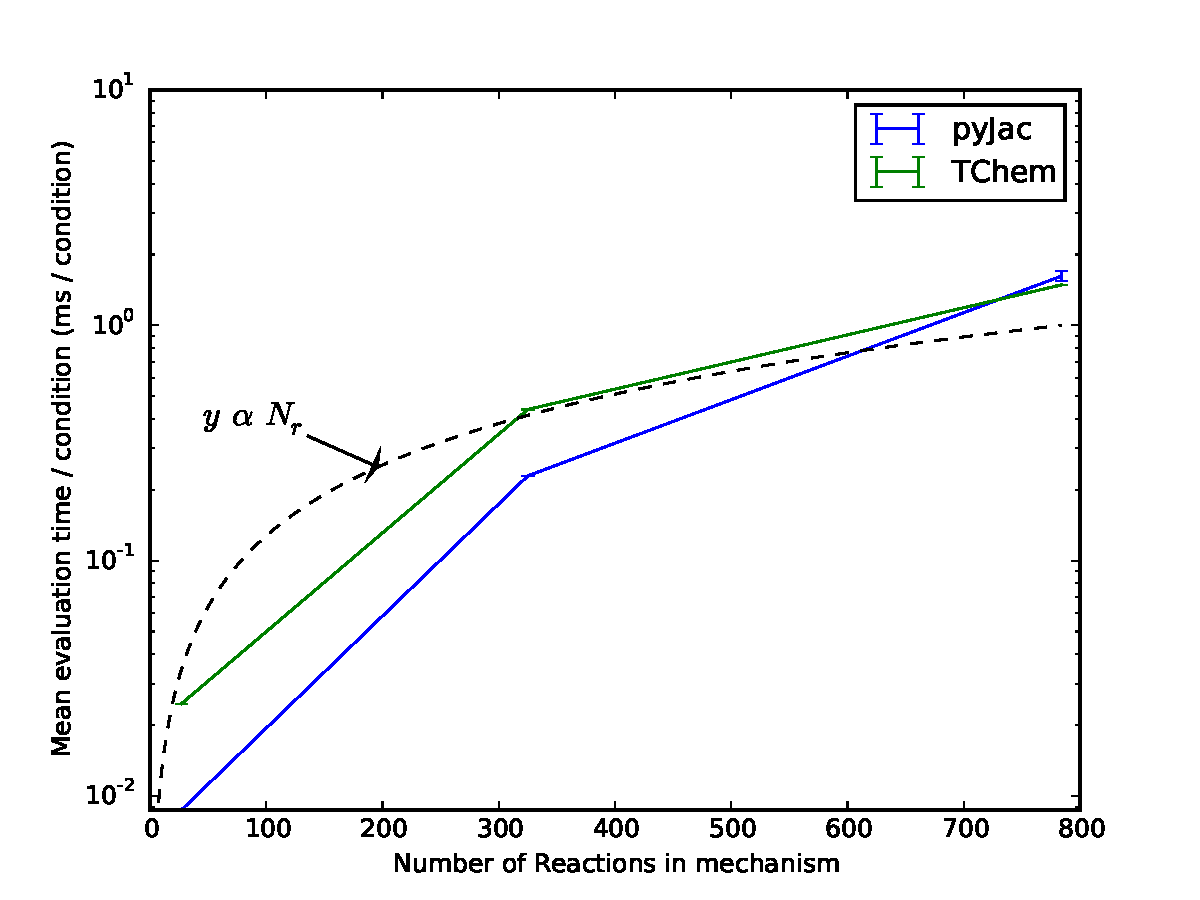
\includegraphics[width=0.75\textwidth]{cpu_norm.pdf}
    \caption{Comparison of \texttt{pyJac} and \texttt{TChem} Jacobian matrix evaluation times for the various kinetic models. 
    The dashed line indicates a linear scaling of evaluation time with the number of reactions in the mechanism.}
    \label{F:cpu_perf}
\end{figure}

\begin{table}[tbp]
\centering
\begin{tabular}{@{}l l@{}}
\toprule
Mechanism & $\bar{R}_{\texttt{TChem}} / \bar{R}_{\texttt{pyJac}}$ \\
\midrule
\ce{H2}\slash \ce{CO} & 2.82 \\
GRI-Mech 3.0 &  1.91 \\
USC Mech II &  0.92 \\
\bottomrule
\end{tabular}
\caption{Ratio of Jacobian matrix evaluation times for \texttt{TChem} and \texttt{pyJac}. 
$\bar{R}$ indicates the mean evaluation time.}
\label{t:cpu_comp}
\end{table}

Figure~\ref{F:gpu_perf} presents the performance of the GPU Jacobian matrix implementations.
Figure~\ref{F:gpu_mean} plots the mean runtime of the GPU Jacobian matrix evaluations against the number of conditions---i.e., the number of thermochemical composition states, with one Jacobian matrix evaluated per state.
As the number of conditions increases, the GPU becomes fully utilized and the growth rate of the evaluation time begins increasing linearly (here displayed on a log-log plot).
This thread saturation point occurs at nearly the same number of conditions for each model.
Figure~\ref{F:gpu_norm} shows the longest evaluation time---normalized by the number of conditions---for each kinetic model plotted against the number of reactions.
As with the CPU matrix evaluations shown in Fig.~\ref{F:cpu_perf}, we observed a slight superlinear scaling of the performance with number of reactions.

\begin{figure}[tbp]
    \centering
    \begin{subfigure}{0.5\textwidth}
        \centering
        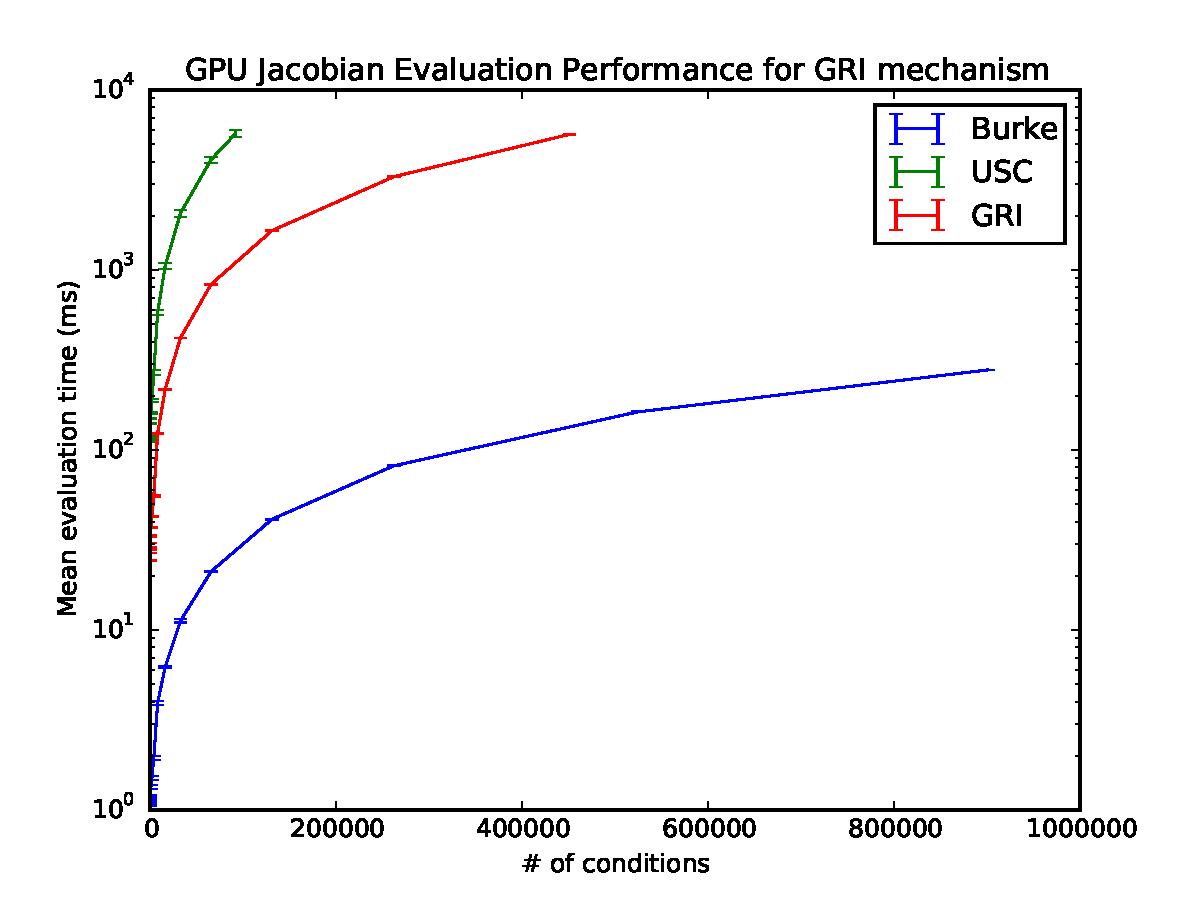
\includegraphics[width=\textwidth]{gpu.pdf}
        \caption{Mean GPU runtime versus the number of conditions evaluated.}
        \label{F:gpu_mean}
    \end{subfigure}%
    ~
    \begin{subfigure}{0.5\textwidth}
        \centering
        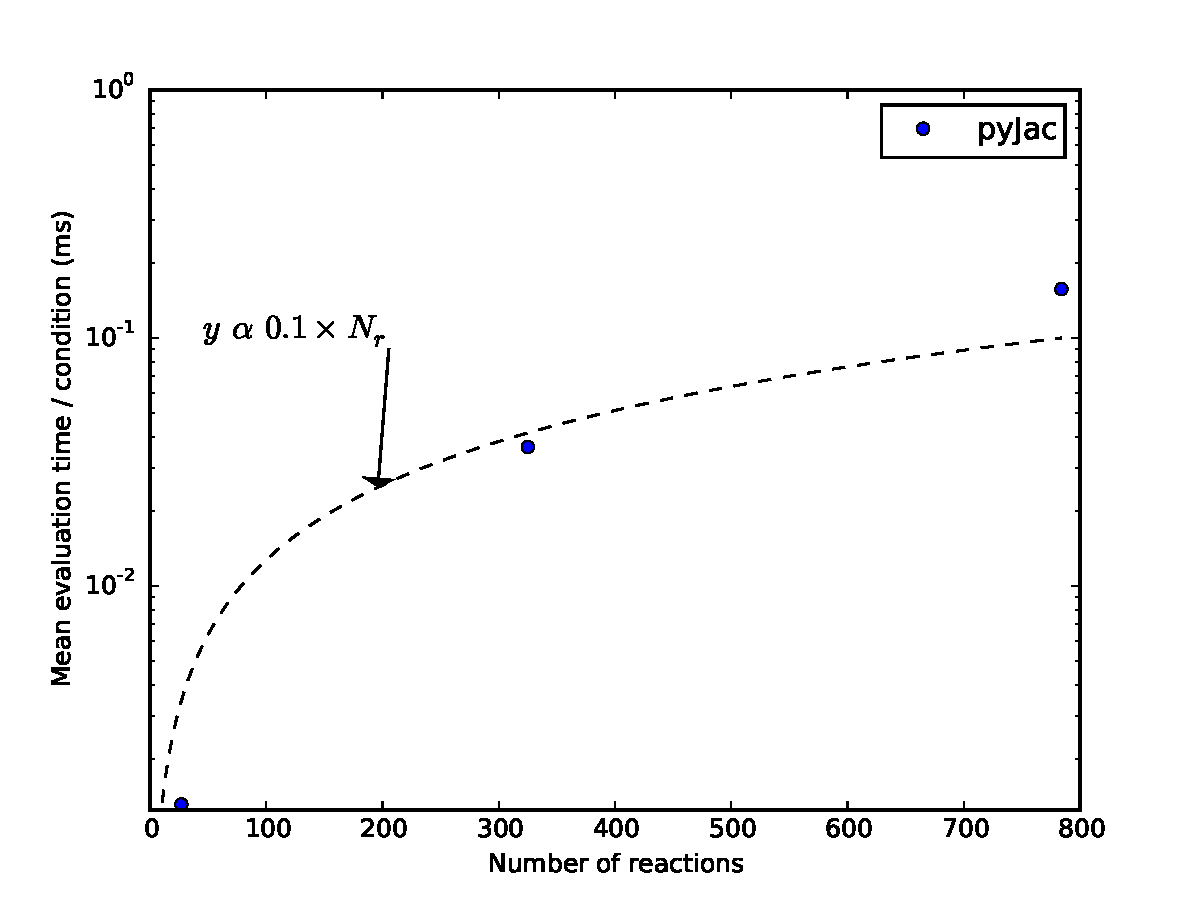
\includegraphics[width=\textwidth]{gpu_norm.pdf}
        \caption{Normalized GPU runtime versus the number of reactions in the mechanism.}
        \label{F:gpu_norm}
    \end{subfigure}
    \caption{Performance of the GPU-based \texttt{pyJac} Jacobian evaluation.
    Note the logarithmic scales of the y-axes.}
    \label{F:gpu_perf}
\end{figure}

The results presented above raise a number of questions that warrant further study, particularly for the CPU implementations.
The near-linear scaling of \texttt{pyJac} matrix evaluation time with number of reactions in the kinetic models conforms with the proposed scaling in the literature~\cite{Lu:2009gh}.
However, while \texttt{pyJac} outperforms \texttt{TChem} by a factor of 2.8 for the \ce{H2}\slash\ce{CO} mechanism, the performance ratio between them drops with increasing kinetic model size, with \texttt{pyJac} performing worse for USC Mech II.
This trend implies that producing custom CPU source code files for evaluating Jacobian matrices may not be optimal for larger kinetic models, likely due to the large files required.
For example, the Jacobian evaluation subroutine for USC Mech II comprises \num{363832} total lines spread across 17 files (not including the supporting files for, e.g., species and reaction rate evaluations)---attempting to incorporate the entire matrix evaluation in a single file resulted in the \texttt{gcc} 4.4.7 compiler crashing.
This calls into question our original hypothesis that hard-coded Jacobian matrix evaluation subroutines would always outperform a loop\slash branch-based implementation, and merits further investigation.

%\subsection{Jacobian matrix sparsity}
%\label{s:sparsity}

%%%%%%%%%%%%%%%%%%%%%%%%%%%%%%%%%%%%%%%%%%%%%%%%%%%%%%%%%%%%%%%%%%%%%
\section{Conclusions}
\label{S:conclusions}

This work developed the theory behind an analytic Jacobian matrix evaluation approach for constant-pressure chemical kinetics, including new derivations of partial derivatives with respect to modern reaction pressure-dependence formulations.
In addition, strategies for efficient evaluation were detailed, including reordering matrix element evaluations in order to enable the reuse of temporary products.
The presented methodology was implemented in the open-source software package \texttt{pyJac}~\cite{Niemeyer:2015im}, which generates custom source code files for evaluating chemical kinetics Jacobian matrices on both CPU and GPU systems.
Finally, the correctness of the resulting Jacobian matrices was established, and the performance of the CPU and GPU matrix evaluation subroutines investigated.

Planned work includes further validation of \texttt{pyJac} using larger and more complex chemical kinetic models, including the butanol mechanism of Merchant et al.~\cite{Merchant:2013kz,Hansen:2013fe}, with 372 species and 8723 reversible reactions.
In addition, future versions of \texttt{pyJac} will include the option of assuming constant-volume combustion, and support for generating Fortran and Matlab source code.
Finally, further study will be performed into the benefits of the current hard-coded, compiled Jacobian evaluation subroutine approach versus a loop\slash branch-based approach, in order to determine how to obtain the best performance scaling with kinetic model size.

%%%%%%%%%%%%%%%%%%%%%%%%%%%%%%%%%%%%%%%%%%%%%%%%%%%%%%%%%%%%%%%%%%%%%%
\section*{Acknowledgments}

This material is based upon work supported by the National Science Foundation under Grant Nos.~1535065 and 1534688.

\pagebreak


%% The Appendices part starts with the command \appendix;
%% appendix sections are then done as normal sections
\appendix


\section{Proof of partial derivative of pressure}
\label{A:pres_deriv}
%%%%%%%%%%%%%%%%%%%%%%%%%%%%%%%%%%%%%

{\allowdisplaybreaks \begin{IEEEeqnarray}{rCl}
\dydx{p}{Y_j} &=& \ddx{Y_j} \left( \mathcal{R} \sum_{k=1}^{N_{\text{sp}}} [X_k] \right) = \mathcal{R} T \sum_{k=1}^{N_{\text{sp}}} \dydx{[X_k]}{Y_j} \nonumber \\
  &=& \mathcal{R} T \sum_{k=1}^{N_{\text{sp}}} \left( -[X_k] \frac{W}{W_k} + \delta_{kj} \frac{\rho}{W_k} \right) \nonumber \\
  &=& -\mathcal{R} T \frac{W}{W_j} \sum_{k=1}^{N_{\text{sp}}} [X_k] + \mathcal{R} T \rho \sum_{k=1}^{N_{\text{sp}}} \frac{\delta_{kj}}{W_k} \nonumber \\
  &=& -p \frac{W}{W_j} + \mathcal{R} T \rho \frac{1}{W_j} = -p \frac{W}{W_j} + p \frac{W}{W_j} \nonumber \\
\therefore \dydx{p}{Y_j} &=& 0 \;.
\end{IEEEeqnarray}}%


%%%%%%%%%%%%%%%%%%%%%%%%%%%%%%%%%%%%%
\section{Partially stirred reactor implementation}
\label{A:pasr}

Here, we describe our partially stirred reactor (PaSR) implementation for completeness, based on prior descriptions~\cite{Correa:1993ud,Chen:1997ta,Pope:1997wu,Bhave:2004hc,Ren:2004fz,Ren:2014cd}.
The reactor model consists of an even number \emph{N} of particles, each with a time-varying composition $\phi (t)$.
Unlike the composition vector described previously (Eq.~\eqref{e:vars}), here we use mixture enthalpy and species mass fractions:
\begin{equation}
\phi = \left \lbrace h, Y_1, Y_2, \dotsc, Y_{N_{\text{sp}}} \right \rbrace^{\intercal} \;.
\end{equation}
At discrete time steps of size $\Delta t$, events including inflow, outflow, and pairing cause certain particles to change composition; between these time steps, mixing and reaction fractional steps separated by step size $\Delta t_{\text{sub}}$ evolve the composition of all particles.

Inflow and outflow events at the discrete time steps comprise the inflow stream compositions replacing the compositions of $N \Delta t / \tau_{\text{res}}$ randomly selected particles, where $\tau_{\text{res}}$ is the residence time.
For premixed combustion cases, the inflow streams consist of a fresh fuel\slash air mixture stream at a specified temperature and equivalence ratio and a pilot stream consisting of the adiabatic equilibrium products of the fresh mixture stream, with the mass flow rates of these two streams in a ratio of $0.95 \mathbin{:} 0.05$.
Non-premixed cases consist of three inflow streams: air, fuel, and a pilot consisting of the adiabatic equilibrium products of a stoichiometric fuel\slash air mixture at the same unburned temperature as the first two streams; the mass flow rates of these streams occur in a ratio of $0.85 \mathbin{:} 0.05 \mathbin{:} 0.1$. 
Then, $\frac{1}{2} N \Delta t / \tau_{\text{pair}}$ pairs of particles not including the inflowing particles, where $\tau_{\text{pair}}$ is the pairing timescale, are randomly selected for pairing and then randomly shuffled with the inflowing particles to exchange partners.

Although multiple mixing models exist~\cite{Ren:2004fz}, the current mixing fractional step consists of a pair of two particles $p$ and $q$ exchanging compositional information and evolving by
\begin{align}
\frac{d \phi^p}{dt} &= - \frac{ \phi^p - \phi^q }{ \tau_{\text{mix}} } \quad \text{and} \\
\frac{d \phi^q}{dt} &= - \frac{ \phi^q - \phi^p }{ \tau_{\text{mix}} } \;,
\end{align}
where $\tau_{\text{mix}}$ is a characteristic mixing timescale.
The analytical solution to this system of equations determines the particle compositions $\phi^p$ and $\phi^q$ after a mixture fractional step:
\begin{align}
\phi^p &= \phi^p_0 - \alpha \;, \\
\phi^q &= \phi^q_0 + \alpha \;, \text{ and} \\
\alpha &= \frac{ \phi^p_0 - \phi^q_0 }{2} \left[1 - \exp \left( \frac{-2 \delta t}{\tau_{\text{mix}}} \right) \right] \;,
\end{align}
where $\phi^p_0$ and $\phi^q_0$ are the particle compositions at the beginning of the mixture fractional step.
The reaction fractional step consists of the enthalpy evolving by
\begin{equation}
\frac{dh}{dt} = \frac{-1}{\rho} \sum_{k=1}^{N_{\text{sp}}} h_k W_k \dot{\omega}_k
\end{equation}
and the species mass fractions evolving according to Eq.~\eqref{e:dTdt}.
However, in practice our implementation handles the reaction fractional step by advancing in time a Cantera~\cite{Goodwin:2014aa} \texttt{ReactorNet} that contains a \texttt{IdealGasConstPressureReactor} object, rather than integrating the above equations directly.

The time integration scheme implemented in our approach determines the discrete time step between inflow\slash outflow and pairing events and the sub-time step size separating mixing\slash reaction fractional steps, both held constant in the current implementation, via
\begin{align}
\Delta t &= 0.1 \, \min \left( \tau_{\text{res}} , \tau_{\text{pair}} \right) \; \text{and} \\
\Delta t_{\text{sub}} &= 0.04 \, \tau_{\text{mix}} \;,
\end{align}
adopted from Pope~\cite{Pope:1997wu}.

\begin{figure}[tbp]
\centering
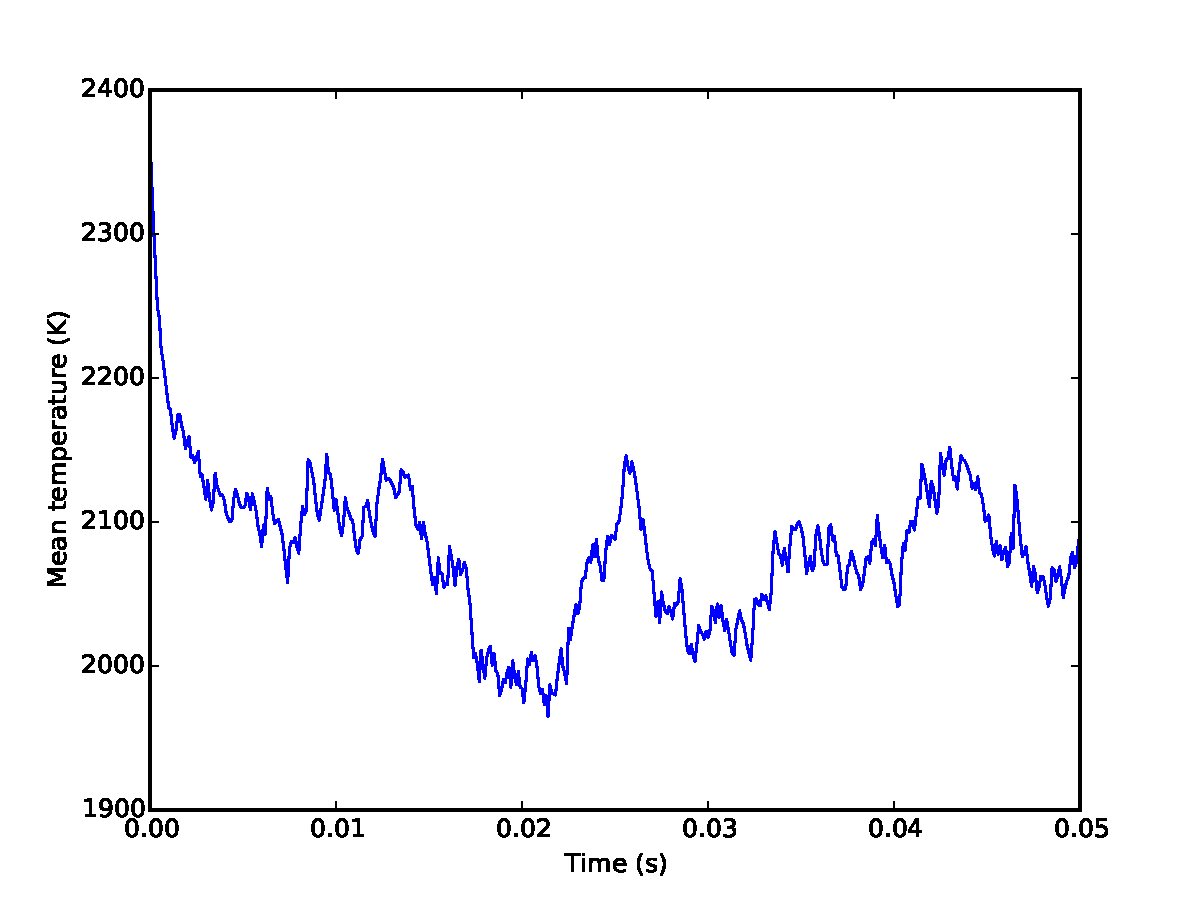
\includegraphics[width=.75\textwidth]{CH4_600K_1atm_mean_temperature.pdf}
\caption{Mean temperature of premixed PaSR combustion for stoichiometric methane\slash air with an unburned temperature of \SI{600}{\kelvin} and at \SI{1}{\atm}, $\tau_{\text{res}} = \SI{5}{\milli\second}$, $\tau_{\text{mix}} = \tau_{\text{pair}} = \SI{1}{\milli\second}$, and using 100 particles.}
\label{F:ch4_meantemp}
\end{figure}

\begin{figure}[tbp]
\centering
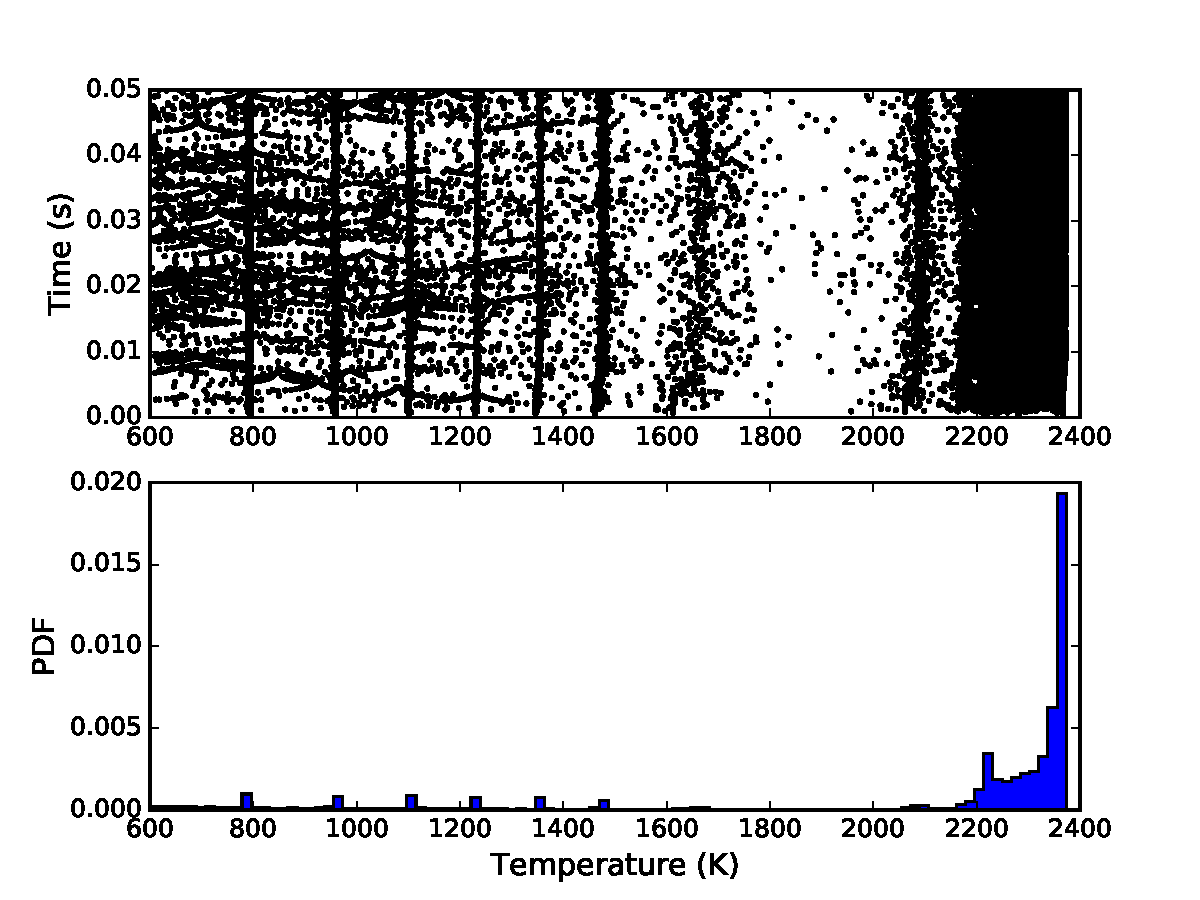
\includegraphics[width=.75\textwidth]{CH4_600K_1atm_particle_temperature.pdf}
\caption{Scatterplot of temperature over time (top) and PDF of temperature (bottom) of premixed PaSR combustion for stoichiometric methane\slash air with an unburned temperature of \SI{600}{\kelvin} and at \SI{1}{\atm}, $\tau_{\text{res}} = \SI{5}{\milli\second}$, $\tau_{\text{mix}} = \tau_{\text{pair}} = \SI{1}{\milli\second}$, and using 100 particles.}
\label{F:ch4_particle_temp}
\end{figure}

Figures~\ref{F:ch4_meantemp} and \ref{F:ch4_particle_temp} demonstrate sample results from premixed PaSR combustion of methane\slash air, using GRI-Mech 3.0~\cite{smith_gri-mech_30}; Fig.~\ref{F:ch4_meantemp} shows the mean temperature evolution over time, while Fig.~\ref{F:ch4_particle_temp} shows the temperature distribution among all particles.
Although a large number of particles reside near the equilibrium temperature of \SI{2367}{\kelvin}, the wide distribution in particle states is evident.

%%%%%%%%%%%%%%%%%%%%%%%%%%%%%%%%%%%%%%%%%%%%%%%%%%%%%%%%%%%%%%%%%%%%%
%% Place the appropriate \bibliography command here.
%% Notice that the class file automatically sets \bibliographystyle
%% and also names the section correctly.
%%%%%%%%%%%%%%%%%%%%%%%%%%%%%%%%%%%%%%%%%%%%%%%%%%%%%%%%%%%%%%%%%%%%%

\bibliography{refs}
\bibliographystyle{elsarticle-num}
%\bibliographystyle{elsarticle-num-CNF}


\end{document}
